\documentclass[twoside]{article}
\author{Michele Mazza}
% Pacchetti di Codifica e Lingua
\usepackage[utf8]{inputenc}
\usepackage[T1]{fontenc}
\usepackage[italian]{babel}

% Pacchetti Grafici e Diagrammi
\usepackage{graphicx}
\usepackage{tikz}
\usepackage{tikz-3dplot}
\usetikzlibrary{angles,quotes,arrows.meta, positioning, 3d, matrix, calc}
\usepackage{pgfplots}
\pgfplotsset{compat=1.18}

% Pacchetti Matematici
\usepackage{amsmath, amssymb}

% Scegliere tra amsthm e ntheorem
%\usepackage{ntheorem}
% Se si preferisce amsthm, commentare la riga sopra e decommentare la seguente
\usepackage{amsthm}
\usepackage{cancel}

% Pacchetti per Tabelle e Unità di Misura
\usepackage{geometry}
\usepackage{siunitx}
\usepackage{booktabs}
\usepackage{tabularx}
\usepackage{colortbl}
\usepackage{adjustbox}

% Pacchetti per Layout e Formattazione
\usepackage{fancyhdr}
\usepackage{float}
\usepackage{microtype}
\usepackage{multicol}

% Altri Pacchetti Utili
\usepackage{mdframed}
\usepackage{animate}
\usepackage{ulem}
\usepackage{eurosym}

% Pacchetto enumitem
\usepackage{enumitem}

% Definizioni dei Colori e Comandi Personalizzati
\definecolor{lightblue}{HTML}{9cd8fc}
\definecolor{myblue}{HTML}{139FE9}
\definecolor{myblack}{HTML}{303030}
\definecolor{mygray}{HTML}{787878}
\definecolor{mywhite}{HTML}{c7c7c7}
\newcommand{\norm}[1]{\left\lVert#1\right\rVert}

% Ambienti Personalizzati
% Usa \theoremstyle e \theorembodyfont come necessario
\newmdtheoremenv[
    backgroundcolor=orange!10,
    linecolor=myblue,
    linewidth=0pt,
    leftmargin=0pt,
    rightmargin=0pt,
    innerleftmargin=10pt,
    innerrightmargin=10pt,
    innertopmargin=10pt,
    innerbottommargin=10pt,
    nobreak
]{curiosity}{Curiosità}

\newmdtheoremenv[
    font=\normalfont\small,
    linewidth=0pt,
    innerleftmargin=10pt,
    innerrightmargin=10pt,
]{example}{Esempio}

\newmdtheoremenv[
  backgroundcolor=lightblue,
  linecolor=myblue,
  linewidth=1.5pt,
  innertopmargin=10pt,
  innerbottommargin=10pt,
  innerrightmargin=10pt,
  innerleftmargin=10pt,
  nobreak
]{theorem}{Teorema}

\newmdtheoremenv[
  backgroundcolor=gray!10,
  linewidth=0pt,
  innertopmargin=-5pt,
  innerbottommargin=5pt,
  innerrightmargin=10pt,
  innerleftmargin=10pt,
  nobreak
]{definition}{Definizione}

\newmdtheoremenv[
  backgroundcolor=gray!10,
  linecolor=myblue,
  linewidth=1.5pt,
  innertopmargin=-5pt,
  innerbottommargin=5pt,
  innerrightmargin=10pt,
  innerleftmargin=10pt,
  nobreak
]{proposition}{Proposizione}


% Configurazioni di fancyhdr
\pagestyle{fancy}
\fancyhf{}
\fancyhead[RE,RO]{\nouppercase{\rightmark}}
\fancyfoot[C]{\thepage}
\renewcommand{\headrulewidth}{0.0pt}
\renewcommand{\footrulewidth}{0pt}
\geometry{a4paper, left=20mm, right=20mm, top=20mm, bottom=20mm}

\usepackage{titlesec} % Pacchetto per personalizzare i titoli delle sezioni

% Definisci i colori per le diverse sezioni
\titleformat{\section}
{\color{black}\normalfont\Large\bfseries}
{\thesection}{1em}{}

\titleformat{\subsection}
{\color{red}\normalfont\large\bfseries}
{\thesubsection}{1em}{}

\titleformat{\subsubsection}
{\color{blue}\normalfont\normalsize\bfseries}
{\thesubsubsection}{1em}{}

% Pacchetti Aggiuntivi
\usepackage{xparse,array}

% Pacchetto Hyperref (inserito per ultimo)
\usepackage{hyperref}

\begin{document}
\title{Fisica Generale T-A}
\maketitle
\hrulefill
\section{Intro}
\rule{\linewidth/2}{0.5pt}
\subsection{Vettori}
\subsubsection{Somma}
\begin{equation}
  \boxed{\vec{a} + \vec{b} = \vec{c}}
\end{equation}
\begin{equation}
  \boxed{(a_x, a_y) + (b_x, b_y) = (a_x + b_x, a_y + b_y) = (c_x, c_y)}
\end{equation}
\begin{figure}[H]
  \centering
  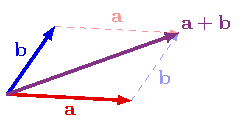
\includegraphics{src/vector/image3.pdf}
  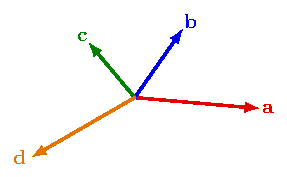
\includegraphics{src/vector/image4.pdf}
  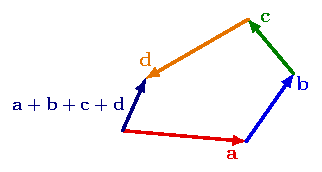
\includegraphics{src/vector/image5.pdf}
\end{figure}
\subsubsection{Prodotto per uno scalare}
\begin{equation}
  \boxed{\lambda \cdot \vec{a}}
\end{equation}
\begin{equation}
  \boxed{\lambda \cdot (a_x, a_y) = (\lambda \cdot a_x, \lambda \cdot a_y)}
\end{equation}
\subsubsection{Prodotto scalare}
Da un numero
\begin{equation}
  \boxed{\vec{a} \cdot \vec{b} = |a| \cdot |b| \cdot \cos{\theta}}
\end{equation}
\begin{equation}
  \boxed{(a_x, a_y) \cdot (b_x, b_y) = a_x \cdot b_x + a_y \cdot b_y}
\end{equation}
\subsubsection{Prodotto vettoriale}
Da un vettore
\begin{equation}
  \boxed{\vec{a} \times \vec{b} = |a| \cdot |b| \cdot \sin{\theta} = \vec{c}}
\end{equation}
\begin{equation}
  \boxed{\vec{a} \times \vec{b} = det \begin{pmatrix}
      \hat{i} & \hat{j} & \hat{k} \\
      a_x     & a_y     & a_z     \\
      b_x     & b_y     & b_z
    \end{pmatrix}}
\end{equation}
Sarrus (solo 3 x 3)
\begin{equation*}
  \vec{a} \times \vec{b}  = \begin{tikzpicture}[>=stealth, baseline=-0.5ex]
    \matrix [
      matrix of math nodes,
      column sep=1em,
      row sep=1em
    ] (sarrus) {
      \hat{i_{x}} & \hat{j_{y}} & \hat{k_{z}} & \hat{i_{x}} & \hat{j_{y}} \\
      a_x                                 & a_y                                 & a_z                                 & a_x                                 & a_y                                 \\
      b_x                                 & b_y                                 & b_z                                 & b_x                                 & b_y                                 \\
    };
    \path ($(sarrus-1-1.north west)-(0.5em,0)$) edge ($(sarrus-3-1.south west)-(0.5em,0)$)
    ($(sarrus-1-3.north east)+(0.5em,0)$) edge ($(sarrus-3-3.south east)+(0.5em,0)$)
    (sarrus-1-1)                          edge[red]             (sarrus-2-2)
    (sarrus-2-2)                          edge[->, red]         (sarrus-3-3)
    (sarrus-1-2)                          edge[red]             (sarrus-2-3)
    (sarrus-2-3)                          edge[->, red]         (sarrus-3-4)
    (sarrus-1-3)                          edge[red]             (sarrus-2-4)
    (sarrus-2-4)                          edge[->, red]         (sarrus-3-5)
    (sarrus-3-1)                          edge[dashed, blue]    (sarrus-2-2)
    (sarrus-2-2)                          edge[->,dashed, blue] (sarrus-1-3)
    (sarrus-3-2)                          edge[dashed, blue]    (sarrus-2-3)
    (sarrus-2-3)                          edge[->,dashed, blue] (sarrus-1-4)
    (sarrus-3-3)                          edge[dashed, blue]    (sarrus-2-4)
    (sarrus-2-4)                          edge[->,dashed, blue] (sarrus-1-5);
    \foreach \c in {1,2,3} {\node[anchor=south] at (sarrus-1-\c.north) {$\textcolor{red}{+}$};};
    \foreach \c in {1,2,3} {\node[anchor=north] at (sarrus-3-\c.south) {$\textcolor{blue}{-}$};};
  \end{tikzpicture} = (\hat{i} \cdot a_y \cdot b_z) + (\hat{j} \cdot a_z \cdot b_x) + (\hat{k} \cdot a_x \cdot b_y) - (\hat{i} \cdot a_z \cdot b_y) - (\hat{j} \cdot a_x \cdot b_z) - (\hat{k} \cdot a_y \cdot b_x)
\end{equation*}
Per le matrici 2 x 2
\begin{equation*}
  \vec{a} \times \vec{b} = det \begin{pmatrix}
    a_x & a_y \\
    b_x & b_y
  \end{pmatrix} = a_x \cdot b_y - a_y \cdot b_x
\end{equation*}
\subsubsection{Versore}
\begin{equation}
  \boxed{\hat{u} = \frac{\vec{a}}{|a|}}
\end{equation}
\begin{equation*}
  |\hat{u}| = 1
\end{equation*}
\begin{equation*}
  \vec{a} = |\vec{a}|\ \hat{u}
\end{equation*}
\begin{equation*}
  \vec{a} = a_u\ \hat{u}
\end{equation*}
\begin{figure}[H]
  \centering
  \tdplotsetmaincoords{70}{120}
  \begin{tikzpicture}[tdplot_main_coords, scale=0.5]
    % valori massimi degli assi cartesiani
    \def\xMax{7}
    \def\yMax{7}
    \def\zMax{4}
    % a
    \def\ax{7}
    \def\ay{7}
    \def\az{7}
    % b
    \def\bx{3}
    \def\by{3}
    \def\bz{3}
    % c
    \def\cx{0}
    \def\cy{0}
    \def\cz{3}
    \draw[-latex, thick] (-\xMax,0,0) -- (\xMax,0,0) node[anchor=north east]{\(x\)};
    \draw[-latex, thick] (0,-\yMax,0) -- (0,\yMax,0) node[anchor=west]{\(y\)};
    \draw[-latex, thick] (0,0,-\zMax/2) -- (0,0,\zMax) node[anchor=south]{\(z\)};
    \draw[fill=mygray, opacity=0.05] (-\xMax,-\yMax,0) -- (\xMax,-\yMax,0) -- (\xMax,\yMax,0) -- (-\xMax,\yMax,0) -- cycle;
    \draw[-stealth, ultra thick, blue] (0,0,0) -- (\ax,\ay,\az) node[anchor=north west]{\(\vec{a}\)};
    \draw[-stealth, ultra thick, red] (0,0,0) -- (\bx,\by,\bz) node[anchor=south east]{\(\hat{u}\)};
  \end{tikzpicture}
\end{figure}
Per la terna cartesiana si usa spesso la notazione \(\hat{i}, \hat{j}, \hat{k}\) per indicare i versori lungo gli assi cartesiani \(x, y, z\)
\begin{figure}[H]
  \centering
  \tdplotsetmaincoords{70}{120}
  \begin{tikzpicture}[tdplot_main_coords, scale=0.5]
    % valori massimi degli assi cartesiani
    \def\xMax{7}
    \def\yMax{7}
    \def\zMax{4}
    % a
    \def\ax{3}
    \def\ay{0}
    \def\az{0}
    % b
    \def\bx{0}
    \def\by{3}
    \def\bz{0}
    % c
    \def\cx{0}
    \def\cy{0}
    \def\cz{3}
    \draw[-latex, thick] (-\xMax,0,0) -- (\xMax,0,0) node[anchor=north east]{\(x\)};
    \draw[-latex, thick] (0,-\yMax,0) -- (0,\yMax,0) node[anchor=west]{\(y\)};
    \draw[-latex, thick] (0,0,-\zMax/2) -- (0,0,\zMax) node[anchor=south]{\(z\)};
    \draw[fill=mygray, opacity=0.05] (-\xMax,-\yMax,0) -- (\xMax,-\yMax,0) -- (\xMax,\yMax,0) -- (-\xMax,\yMax,0) -- cycle;
    \draw[-stealth, ultra thick, blue] (0,0,0) -- (\ax,\ay,\az) node[anchor=north west]{\(\hat{i}\)};
    \draw[-stealth, ultra thick, red] (0,0,0) -- (\bx,\by,\bz) node[anchor=south east]{\(\hat{j}\)};
    \draw[-stealth, ultra thick, orange] (0,0,0) -- (\cx,\cy,\cz) node[anchor=west]{\(\hat{k}\)};
  \end{tikzpicture}
\end{figure}
\subsubsection{Funzione vettoriale}
\begin{equation}
  \boxed{\vec{r}(t) = x\hat{i}+y\hat{j}+z\hat{k} = (x(t), y(t), z(t))}
\end{equation}
\begin{figure}[H]
  \centering
  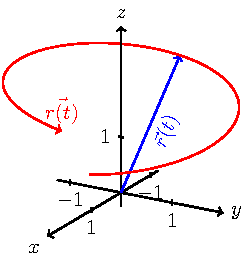
\includegraphics{src/vector/image6.pdf}
\end{figure}

\subsubsection{Derivata di una funzione vettoriale}
\begin{equation}
  \boxed{\frac{d\ \vec{r}(t)}{dt} = \frac{d(x(t), y(t), z(t))}{dt} = (\frac{dx}{dt}, \frac{dy}{dt}, \frac{dz}{dt}) = \vec{v}(t)}
\end{equation}
\begin{figure}[H]
  \centering
  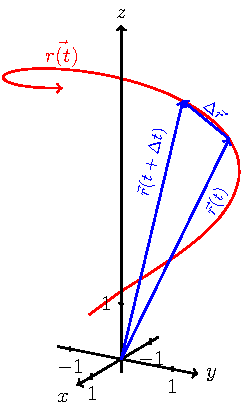
\includegraphics{src/vector/image7.pdf}
\end{figure}
Posso riscrivere la derivata di una funzione vettoriale in termini dei versori e delle componenti
\begin{equation*}
  \frac{d\ \vec{r}(t)}{dt} = \frac{d\left(\ r(t) \cdot \hat{u}_r(t)\ \right)}{dt}
\end{equation*}
\begin{equation*}
  \frac{d\left(\ r(t) \cdot \hat{u}_r(t)\ \right)}{dt} =\footnotemark[1] \ \textcolor{blue}{\underline{\frac{d\ r(t)}{dt}\ \hat{u}_r(t)}} + \textcolor{violet}{\uuline{r(t)\ \frac{d\ \hat{u}_r(t)}{dt}}}
\end{equation*}
\begin{align*}
  \textcolor{blue}{\underline{\frac{d\ r(t)}{dt}\ \hat{u}_r(t)}} & \textcolor{blue}{=\ v(t)\ \hat{u}_r(t) = \vec{v}(t)} \\
                                                                 & \textcolor{blue}{= \text{Componente tangenziale}}    \\
                                                                 & \textcolor{blue}{=\ \Vec{T}}                         \\
\end{align*}
\begin{align*}
  \textcolor{violet}{\uuline{r(t)\ \left(\frac{d\ \hat{u}_r(t)}{dt}\right)}} & \textcolor{violet}{= r(t)\  \left(\vec{\omega}(t) \times \hat{u}_r(t)\right)}\footnotemark[2]  \\
                                                                             & \textcolor{violet}{= \vec{\omega}(t) \times \left( r(t) \hat{u}_r(t) \right) }\footnotemark[3] \\
                                                                             & \textcolor{violet}{= \vec{\omega}(t) \times \vec{r}(t) }                                       \\
                                                                             & \textcolor{violet}{=\ \text{Componente radiale}}                                               \\
                                                                             & \textcolor{violet}{=\ \Vec{N}}                                                                 \\
\end{align*}
\begin{equation}
  \boxed{\frac{d\ \vec{r}(t)}{dt} = \vec{v}(t) + \vec{\omega}(t) \times \vec{r}(t)}
\end{equation}
\footnotetext[1]{Derivata di un prodotto : \(\displaystyle (a \cdot b)' = a' \cdot b + a \cdot b'\)}
\footnotetext[2]{Formula di Poisson : \( \displaystyle \frac{d\ \hat{u}(t)}{dt} = \vec{\omega}(t) \times \hat{u}(t)\)}
\footnotetext[3]{Nell'espressione \(\displaystyle r(t) \left(\vec{\omega}(t) \times \hat{u}_r(t)\right)\), il prodotto vettoriale \(\vec{\omega}(t) \times \hat{u}_r(t)\) ha la priorità e viene calcolato per primo, come indicato dalle parentesi. Successivamente, il risultato di questo prodotto vettoriale viene moltiplicato per lo scalare \(r(t)\), risultando in un vettore che mantiene la direzione del prodotto vettoriale ma viene scalato nella magnitudine da \(r(t)\). Questo processo illustra come le operazioni vengano sequenziate matematicamente: le parentesi indicano l'ordine con cui le operazioni devono essere eseguite, confermando che il prodotto vettoriale precede la moltiplicazione scalare.}
\begin{figure}[H]
  \centering
  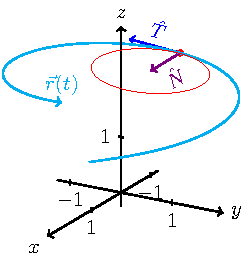
\includegraphics{src/vector/image8.pdf}
\end{figure}
\subsection{Regola della mano destra}
\begin{figure}[H]
  \centering
  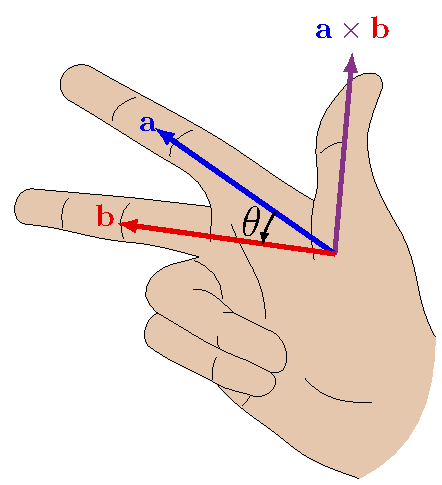
\includegraphics{src/vector/image1.pdf}
  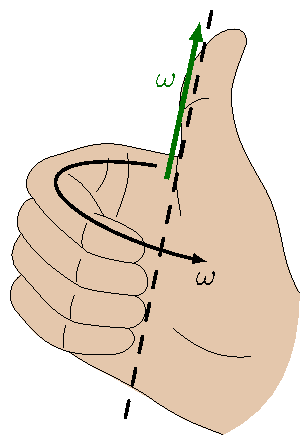
\includegraphics{src/vector/image2.pdf}
\end{figure}
\subsection{Circuitazione}
\begin{equation}
  \boxed{\oint}
\end{equation}
\'E l'integrale di linea, ovvero l'integrale di una funzione vettoriale lungo una curva chiusa. \\
\newpage

\hrulefill
\section{Moti}
\rule{\linewidth/2}{0.5pt}
\subsection{Moto rettilineo uniformemente accelerato}
\subsubsection{Velocità media}
\begin{equation}
  \boxed{\overline{v} = \frac{x_1-x_0}{t_1-t_0} = \frac{\Delta x}{\Delta t}}
\end{equation}
\subsubsection{Velocità istantanea}
\begin{equation}
  \boxed{v(t) = \frac{dx}{dt}}
\end{equation}
\subsubsection{Accelerazione media}
\begin{equation}
  \boxed{\overline{a} = \frac{v_1-v_0}{t_1-t_0} = \frac{\Delta v}{\Delta t}}
\end{equation}
\subsubsection{Accelerazione istantanea}
\begin{equation}
  \boxed{a(t) = \frac{dv}{dt} }
\end{equation}
\subsubsection{Legge oraria}
\begin{equation}
  \boxed{\begin{cases}
      x(t) = x_0 + v_0 \cdot t + \frac{1}{2} \cdot a \cdot t^2 \\
      v(t) = v_0 + a \cdot t
    \end{cases}}
\end{equation}
\subsubsection{Accelerazione senza tempo}
\begin{equation*}
  a = \frac{dv}{dt} \Rightarrow a = \frac{dv}{dt} \cdot \frac{dx}{dx} \Rightarrow a = \frac{dv}{dx} \cdot \frac{dx}{dt} \\
\end{equation*}
Nota che
\begin{equation*}
  v(t) = \frac{dx}{dt}
\end{equation*}
Quindi riprendendo l’equazione precedente
\begin{equation*}
  a = \frac{dv}{dx} \cdot \underline{\frac{dx}{dt}} \Rightarrow a =  \frac{dv}{dx} \cdot \underline{v(t)}
\end{equation*}
\begin{equation*}
  a =  \frac{dv}{dx} \cdot v(t)
\end{equation*}
La tratto come un'equazione differenziale
\begin{equation*}
  a \cdot dx = v(t) \cdot dv
\end{equation*}
Integro entrambi i membri
\begin{equation*}
  \int_{x_0}^{x_1} a \cdot dx = \int_{v_0}^{v_1} v(t) \cdot dv
\end{equation*}
\begin{equation*}
  a \cdot \int_{x_0}^{x_1} dx = \int_{v_0}^{v_1} v(t) \cdot dv
\end{equation*}
\begin{equation*}
  a \cdot (x_1 - x_0) = \frac{1}{2} \cdot v_1^2 - \frac{1}{2} \cdot v_0^2
\end{equation*}
\begin{equation*}
  a \cdot \Delta x = \frac{1}{2} \cdot \Delta v^2
\end{equation*}
\begin{equation}
  \boxed{a = \frac{1}{2} \cdot \frac{\Delta v^2}{\Delta x}}
  \label{eq:accelerazione_senza_tempo}
\end{equation}

\subsection{Moto circolare uniformemente accelerato}
\subsubsection{Velocità angolare}
\begin{equation}
  \boxed{\omega = \frac{d\theta}{dt}}
\end{equation}
Poiché
\begin{equation*}
  d \theta = \frac{ds}{R}
\end{equation*}
\begin{equation*}
  \omega = \frac{ds}{R \cdot dt}
\end{equation*}
\begin{equation}
  \boxed{\omega = \frac{v}{R}}
\end{equation}
\subsubsection{Accelerazione angolare}
\begin{equation}
  \boxed{\alpha = \frac{d\omega}{dt}}
\end{equation}
\begin{equation}
  \boxed{\alpha =\frac{a_t}{R}}
\end{equation}
\subsubsection{Accelerazione centripeta}
Centripeta significa "verso il centro"
\begin{equation}
  \boxed{a_c = \frac{v^2}{R} = \omega^2 \cdot R = v \cdot \omega}
\end{equation}
\subsubsection{Accelerazione tangenziale}
\begin{equation}
  \boxed{a_t = \frac{dv}{dt}}
\end{equation}
\subsubsection{Accelerazione totale}
\begin{equation}
  \boxed{a = \sqrt{a_c^2 + a_t^2}}
\end{equation}
\subsubsection{Legge oraria}
\begin{equation}
  \boxed{\begin{cases}
      \theta(t) = \theta_0 + \omega_0 \cdot t + \frac{1}{2} \cdot \alpha \cdot t^2 \\
      \omega(t) = \omega_0 + \alpha \cdot t
    \end{cases}}
\end{equation}
\subsubsection{Accelerazione angolare senza tempo}
Si ricava come nell'equazione \ref{eq:accelerazione_senza_tempo}
\begin{equation}
  \boxed{\alpha = \frac{1}{2} \cdot \frac{\Delta \omega^2}{\Delta \theta}}
\end{equation}
\begin{figure}[H]
  \centering
  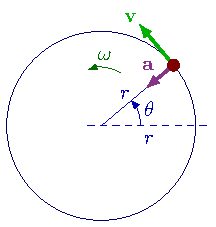
\includegraphics{src/circularmotion/image1.pdf}
  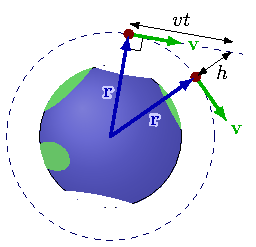
\includegraphics{src/circularmotion/image2.pdf}
  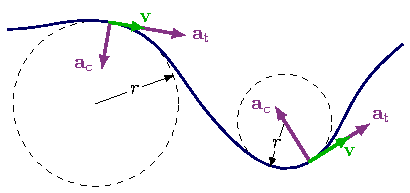
\includegraphics{src/circularmotion/image3.pdf}
\end{figure}
\hrulefill
\subsection{Moto armonico semplice}
\subsubsection{Legge oraria}
\begin{equation}
  \boxed{x(t) = A\cos(\omega t) + B\sin(\omega t)}
\end{equation}
\begin{equation}
  \boxed{x(t) = R\cos(\omega t + \phi)}
\end{equation}
\begin{equation}
  \boxed{x(t) = R\sin(\omega t + \psi)}
\end{equation}
$R = \sqrt{A^2+B^2}$ = ampiezza $[m]$\\
$\omega$ = pulsazione $\frac{[rad]}{[s]}$ ovvero il numero di radianti percorsi in un secondo \\
$\phi \lor \psi$ = la fase iniziale, ovvero l'angolo che forma il vettore con l'asse $x$ al tempo $t = 0$ $[rad]$ \\
$(\omega t + \phi)$ = la fase del moto $[rad]$ \\
Se lo vuoi capire bene bene guarda la dimostrazione che faccio nel pendolo semplice \ref{pendolo_semplice}
\subsubsection{Periodo}
\begin{equation}
  \boxed{T = \frac{2 \pi}{\omega}}
\end{equation}
\subsubsection{Pulsazione}
\begin{equation}
  \boxed{\omega = \frac{2 \pi}{T}}
\end{equation}
\subsubsection{Frequenza}
\begin{equation}
  \boxed{f = \frac{1}{T} = \frac{\omega}{2 \pi}}
\end{equation}
\subsubsection{Velocità}
\begin{equation}
  \boxed{v(t) = -A \cdot \omega \cdot \sin{(\omega \cdot t + \phi_0)}}
\end{equation}
\subsubsection{Accelerazione}
\begin{equation}
  \boxed{a(t) = -A \cdot \omega^2 \cdot \cos{(\omega \cdot t + \phi_0)}}
\end{equation}
\begin{figure}[H]
  \centering
  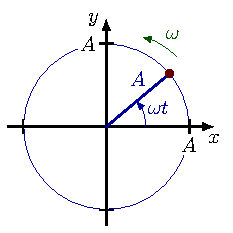
\includegraphics{src/harmonicoscillatorplot/image1.pdf}
  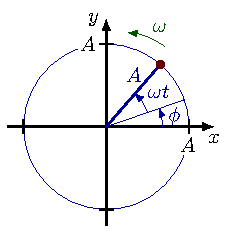
\includegraphics{src/harmonicoscillatorplot/image2.pdf}
\end{figure}
\begin{figure}[H]
  \centering
  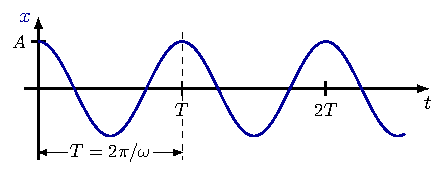
\includegraphics{src/harmonicoscillatorplot/image3.pdf}
  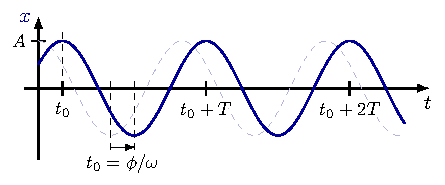
\includegraphics{src/harmonicoscillatorplot/image4.pdf}
  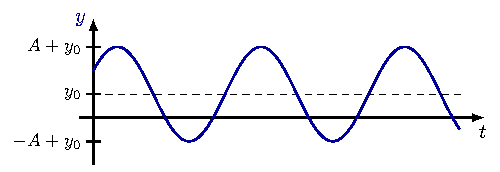
\includegraphics{src/harmonicoscillatorplot/image5.pdf}
  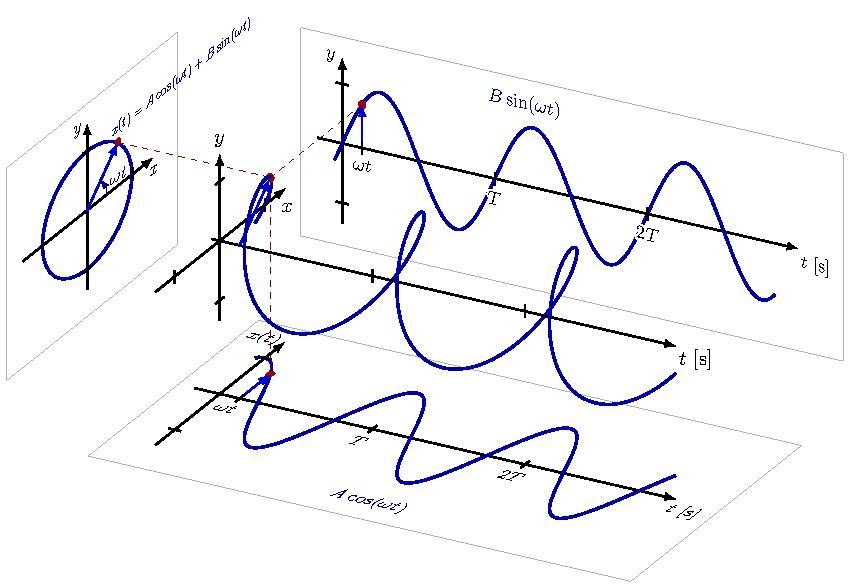
\includegraphics{src/harmonicoscillatorplot/image6.pdf}
\end{figure}
\subsubsection{Forza elastica}
\begin{equation}
  \boxed{w = \sqrt{\frac{k}{m}}}
\end{equation}
\subsubsection{Pendolo semplice}
\begin{equation}
  \boxed{w = \sqrt{\frac{g}{L}}}
\end{equation}
\newpage
\hrulefill

\section{Cinematica del punto materiale}
\subsection{Leggi di Newton}
\subsubsection{Prima legge - Principio d'inerzia}
Un corpo su cui non agiscono forze esterne è in quiete o in moto rettilineo uniforme
\begin{equation}
  \boxed{\sum_{i=1}^{n} \vec{F_i} = 0 \Rightarrow \vec{a} = 0 \Rightarrow \vec{v} = k \lor \vec{v} = 0}
\end{equation}
\subsubsection{Seconda legge - Principio fondamentale della dinamica}
In un sistema di riferimento inerziale, l’accelerazione di un corpo (punto materiale) è sempre
dovuta all’azione di forze. La forza risultante è proporzionale all’accelerazione in ogni
istante tramite una costante scalare di proporzionalità definita massa inerziale
\begin{equation}
  \boxed{\sum_{i=1}^{n} \vec{F_i} = m \cdot \vec{a} = m \cdot \frac{d\vec{v}}{dt} = m \cdot \frac{d^2\vec{x}}{dt^2}}
\end{equation}
\subsubsection{Terza legge - Principio di azione e reazione}
Se un corpo A esercita una forza su un corpo B, allora il corpo B esercita una forza uguale e
contraria sul corpo A (stessa direzione, verso opposto, stessa intensità)
\begin{equation}
  \boxed{\vec{F}_{A \rightarrow B} = - \vec{F}_{B \rightarrow A}}
\end{equation}

\subsubsection{Equilibrio di un punto materiale}
\begin{equation}
  \boxed{\sum_{i=1}^{n} \vec{F_i} = 0}
\end{equation}

\subsection{Forze}
\subsubsection{Forza peso}
\begin{equation}
  \boxed{\vec{F_p} = m \cdot \vec{g}}
\end{equation}
Un corpo poggiato su una piattaforma in grado di muoversi verticalmente ha
\begin{enumerate}
  \item nel caso la piattaforma è ferma o si muove con velocità costante
        \begin{equation*}
          N = F_p = m \cdot g
        \end{equation*}
  \item nel caso la piattaforma si muove con accelerazione verso l’alto
        \begin{equation*}
          N = F_p + F = m \cdot g + m \cdot a
        \end{equation*}
\end{enumerate}

\subsubsection{Reazioni Vincolari}
La reazione vincolare è una forza esercitata da una superficie di contatto su un corpo. Questa forza, nota come forza normale $\vec{F_N}$, agisce perpendicolarmente alla superficie di contatto ed è un vettore perché ha sia magnitudine (intensità) sia direzione.
La forza normale non è sempre uguale e contraria alla forza di attrazione terrestre (forza peso $\vec{F_p}$), che è anch'essa un vettore. La relazione tra $\vec{F_N}$ e $\vec{F_p}$ dipende dalle altre forze che agiscono sul corpo e dalla configurazione del vincolo. In condizioni di equilibrio su una superficie orizzontale, la forza normale bilancia esattamente la componente perpendicolare delle forze esterne, in particolare la forza di gravità:
\begin{equation}
  \boxed{\vec{F_N} = \vec{F_p}} \quad \text{se $\vec{F_p}$ è l'unica forza perpendicolare alla superficie}
\end{equation}
Tuttavia, in situazioni più complesse, la forza normale può differire. Ad esempio, se la superficie su cui poggia il corpo si muove con un'accelerazione $a$ verso l'alto, la magnitudine della forza normale è data da:
\begin{equation}
  \boxed{F_N = m \cdot g + m \cdot a}
\end{equation}
Qui, $F_N$ è usato come uno scalare per rappresentare solo la magnitudine della forza normale, poiché la direzione è implicita (perpendicolare alla superficie).
La condizione di distacco di un corpo dalla superficie si verifica quando la forza normale diventa zero:
\begin{equation}
  \boxed{\vec{F_N} = 0}
\end{equation}
In questo caso, usiamo la notazione vettoriale per indicare che la forza normale (in tutte le direzioni) è assente, il che implica che non c'è più contatto tra il corpo e la superficie.
\begin{figure}[H]
  \centering
  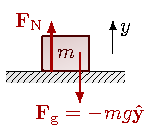
\includegraphics{src/forcenormal/image1.pdf}
  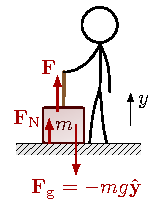
\includegraphics{src/forcenormal/image2.pdf}
  \\
  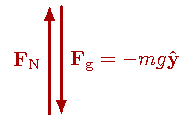
\includegraphics{src/forcenormal/image4.pdf}
  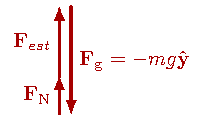
\includegraphics{src/forcenormal/image5.pdf}
  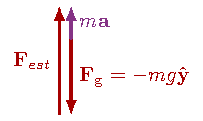
\includegraphics{src/forcenormal/image6.pdf}
  \\
  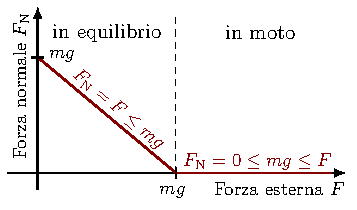
\includegraphics{src/forcenormal/image3.pdf}
\end{figure}

\subsubsection{Densità}
\begin{equation}
  \boxed{\rho = \frac{m}{V}}
\end{equation}

\subsubsection{Forza di attrito}
Se è dinamico $\mu_d$ o statico $\mu_s$, $\mu$ è il coefficiente di attrito, è un numero adimensionale.
\begin{equation}
  \boxed{\vec{F_a} = \mu \cdot \vec{N}}
\end{equation}

\begin{figure}[H]
  \centering
  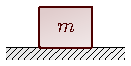
\includegraphics{src/forcefriction/image1.pdf}\\
  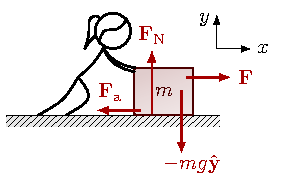
\includegraphics{src/forcefriction/image2.pdf}
  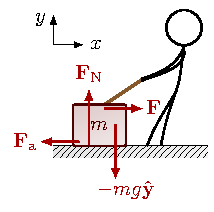
\includegraphics{src/forcefriction/image3.pdf}\\
  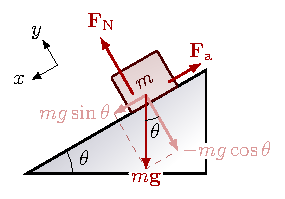
\includegraphics{src/forcefriction/image4.pdf}
  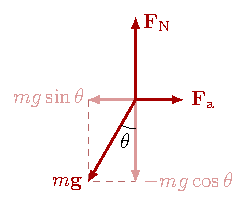
\includegraphics{src/forcefriction/image5.pdf}\\
  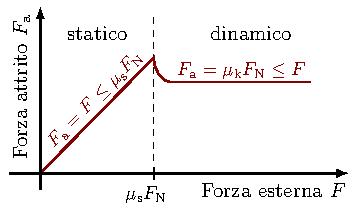
\includegraphics{src/forcefriction/image6.pdf}
\end{figure}

\subsubsection{Forza di attrito viscoso}
Il coefficiente di attrito viscoso, $\eta$, è positivo e si misura in $[kg/s]$\\
\'E una forza che dipende dalla velocità
\begin{equation}
  \boxed{\vec{F_v} = -\eta \cdot \vec{v}}
\end{equation}

Velocità in fluido viscoso
\begin{equation}
  \boxed{v(t) = v_0 \cdot e^{-\frac{\eta}{m} \cdot t}}
\end{equation}
Oppure con la costante di tempo $\tau = \frac{m}{\eta}$
\begin{equation}
  \boxed{v(t) = v_0 \cdot e^{-\frac{t}{\tau}}}
\end{equation}
Velocità limite
\begin{equation}
  \boxed{v_{lim} = g \cdot \tau}
\end{equation}

\subsubsection{Forza centripeta}
\begin{equation}
  \boxed{\vec{F_c} = m \cdot \frac{v^2}{R} = m \cdot \omega^2 \cdot R}
\end{equation}
\begin{figure}[H]
  \centering
  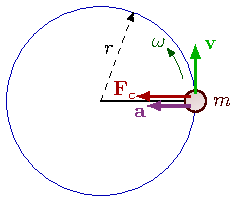
\includegraphics{src/pendulumconical/image2.pdf}
\end{figure}

\subsubsection{Forza elastica}
\begin{equation}
  \boxed{\vec{F_e} = -k \cdot \vec{x}}
\end{equation}
Pulsazione
\begin{equation}
  \boxed{\omega = \sqrt{\frac{k}{m}}}
\end{equation}
Periodo
\begin{equation}
  \boxed{T = 2 \pi \cdot \sqrt{\frac{m}{k}}}
\end{equation}
\begin{figure}[H]
  \centering
  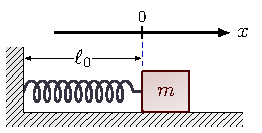
\includegraphics{src/forceelastic/image1.pdf}
  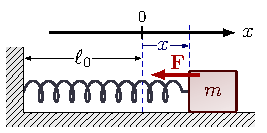
\includegraphics{src/forceelastic/image2.pdf}
  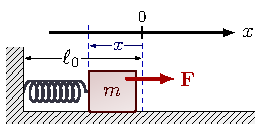
\includegraphics{src/forceelastic/image3.pdf}
\end{figure}
\hrulefill

\subsection{Pendolo semplice}\label{pendolo_semplice}
\begin{figure}[H]
  \centering
  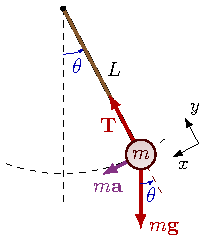
\includegraphics{src/pendulum/image1.pdf}
  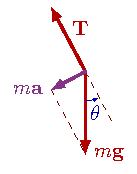
\includegraphics{src/pendulum/image2.pdf}
  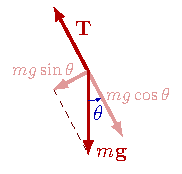
\includegraphics{src/pendulum/image3.pdf}
  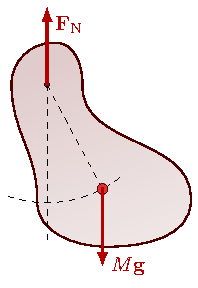
\includegraphics{src/pendulum/image4.pdf}
\end{figure}
\subsubsection{Dimostrazione}
Sono considerati $\theta < 10$ gradi\\
Abbiamo che
\begin{align*}
   & \vec{F_{p \parallel}} = -m \cdot g \cdot \sin{\theta}                         \\
   & \vec{F_{p \perp}}     = -m \cdot g \cdot \cos{\theta}                         \\
   & \vec{T}               = -\vec{F_{p \parallel}} = m \cdot g \cdot \sin{\theta}
\end{align*}
Applicando la seconda legge di Newton\\
Lungo y
\begin{equation*}
  \sum_{i=1}^{n} \vec{F_i}                                     = m \cdot a_c
\end{equation*}
\begin{equation*}
  \vec{F_{p \perp}} + \vec{T}                                  = m \cdot a_c
\end{equation*}
\begin{equation*}
  -m \cdot g \cdot \cos{\theta} + T = m \cdot a_c
\end{equation*}

Lungo x
\begin{equation*}
  \sum_{i=1}^{n} \vec{F_i}                                     = m \cdot a_t
\end{equation*}
\begin{equation*}
  \vec{F_{p \parallel}}                                         = m \cdot a_t
\end{equation*}
\begin{equation*}
  - m \cdot g \cdot \sin{\theta}                                  = m \cdot a_t
\end{equation*}

Metto insieme
\begin{equation*}
  \begin{cases}
    -m \cdot g \cdot \cos{\theta} + T = m \cdot a_c \\
    - m \cdot g \cdot \sin{\theta} = m \cdot a_t
  \end{cases}
\end{equation*}

Nota che
\begin{itemize}
  \item Accelerazione centripeta \begin{equation*}
          a_c = \omega^2 \cdot R
        \end{equation*}
        \begin{equation*}
          a_c = \left(\frac{d\theta}{dt}\right)^2 \cdot R
        \end{equation*}

  \item Accelerazione tangenziale \begin{equation*}
          a_t = \alpha \cdot R
        \end{equation*}
        \begin{equation*}
          a_t = \frac{d^2\theta}{dt^2} \cdot R
        \end{equation*}
\end{itemize}

\begin{equation*}
  \begin{cases}
    \displaystyle -m \cdot g \cdot \cos{\theta} + T = m \cdot \left(\frac{d\theta}{dt}\right)^2 \cdot R \\
    \displaystyle - m \cdot g \cdot \sin{\theta} = m \cdot \frac{d^2\theta}{dt^2} \cdot R
  \end{cases}
\end{equation*}
Semplifco per $m$ e $R$ e inoltre per taylor approssimo $\sin{\theta} \approx \theta$
\begin{equation*}
  \begin{cases}
    \displaystyle -m \cdot g \cdot \cos{\theta} + T = m \cdot \left(\frac{d\theta}{dt}\right)^2 \cdot R \\
    \displaystyle \underline{- \frac{g}{R} \cdot \theta = \frac{d^2\theta}{dt^2}}
  \end{cases}
\end{equation*}
Adesso ci soffermiamo sulla seconda equazione
\begin{equation*}
  \displaystyle - \frac{g}{R} \theta = \frac{d^2\theta}{dt^2}
\end{equation*}
\begin{equation*}
  \displaystyle \frac{d^2\theta}{dt^2} + \frac{g}{R}\theta = 0
\end{equation*}

Abbiamo ottenuto un'equazione differenziale del tipo:
\begin{equation*}
  \frac{d^2\theta}{dt^2} + \frac{g}{L} \theta = 0
\end{equation*}\\
Leggi altrimenti non capisci \(\downarrow\)\\
{\small \textcolor{violet}{
  \textbf{Equazione differenziale lineare omogenea di secondo grado con coefficienti costanti}\\
  La forma generale di tale equazione differenziale è:
  \begin{equation*}
    \frac{d^2x}{dt^2} + kx = 0
  \end{equation*}
  dove :
  \begin{itemize}
    \item \(k\) è una costante positiva
    \item La soluzione generale di un'equazione di questo tipo è ben nota e può essere espressa come una combinazione lineare di funzioni seno e coseno:
          \begin{equation*}
            x(t) = A\cos(\omega t) + B\sin(\omega t)
          \end{equation*}
          \begin{itemize}
            \item \(A\) e \(B\) sono costanti determinate dalle condizioni iniziali del sistema
            \item \(\omega = \sqrt{k}\) rappresenta la frequenza angolare del moto.
          \end{itemize}
    \item Tu adesso ti chiederai si chicco ma come fai dopo?\\
          \textbf{Risposta:} \\
          \begin{itemize}
            \item
                  \begin{equation*}
                    x(t) = A\cos(\omega t) + B\sin(\omega t)
                  \end{equation*}
                  Vale questa io ora ti dico e tu non ti chiedi perché che : \\
                  \begin{itemize}
                    \item \(R = \sqrt( A^2 + B^2 )\)
                    \item \(\phi = \arctan(\frac{B}{A})\)
                    \item \(\psi = \arctan(\frac{A}{B})\)
                  \end{itemize}
                  \begin{equation*}
                    x(t) = A\cos(\omega t) + B\sin(\omega t) = R\cos(\omega t + \phi)
                  \end{equation*}
                  \begin{equation*}
                    x(t) = A\cos(\omega t) + B\sin(\omega t) = R\sin(\omega t + \psi)
                  \end{equation*}
          \end{itemize}
    \item Infine ti dico che scegliere tra seno e coseno per descrivere un'oscillazione è come decidere se osservare un'altalena dal momento in cui parte dal centro o dal suo punto più alto. Seno parte da zero (centro), coseno dal massimo (alto). È solo una questione di da dove preferisci iniziare a guardare il movimento; entrambi raccontano la stessa storia.
  \end{itemize}
}}
Ora tornando al pendolo semplice, identifichiamo \(k = \frac{g}{L}\), quindi \(\omega = \sqrt{\frac{g}{L}}\). Come soluzione generale dell'equazione differenziale, scelgo la funzione
\begin{equation*}
  x(t)= R\sin(\omega t + \psi)
\end{equation*}
dunque tornando a simboli più familiari
\begin{equation*}
  \theta(t) = A\sin(\omega t + \phi)
\end{equation*}
\begin{equation*}
  \theta(t) = A \sin\left(\sqrt{\frac{g}{L}} t + \phi\right)
\end{equation*}
dove \(A\) rappresenta l'ampiezza massima dell'oscillazione e \(\phi\) è la fase iniziale.\\
Non ti fidi che sia vero?\\
\textbf{Risposta:} \\
Sostituiamo sta cosa che abbiamo trovato nella nostra equazione differenziale iniziale
\begin{equation*}
  \frac{d^2\theta(t)}{dt^2} + \frac{g}{L} \theta(t) = 0
\end{equation*}
\begin{equation*}
  \frac{d^2 \left(A \sin\left(\omega t + \phi\right)\right)}{dt^2} + \frac{g}{L} \left(A \sin\left(\omega t + \phi\right)\right) = 0
\end{equation*}
Derivo due volte
\begin{equation*}
  -A \omega^2 \sin\left(\omega t + \phi\right) + \frac{g}{L} A \sin\left(\omega t + \phi\right) = 0
\end{equation*}
Semplifico
\begin{equation*}
  -\cancel{A} \omega^2 \cancel{\sin\left(\omega t + \phi\right)} + \frac{g}{L} \cancel{A} \cancel{\sin\left(\omega t + \phi\right)} = 0
\end{equation*}
\begin{equation*}
  -\omega^2 + \frac{g}{L} = 0
\end{equation*}
\begin{equation*}
  \omega^2 = \frac{g}{L}
\end{equation*}
\begin{equation*}
  \omega = \sqrt{\frac{g}{L}}
\end{equation*}
Non c'è \(\pm\) poiché \(g\) è sempre maggiore di 0 e pure \(L\).
\subsubsection{Formule}
Leggi orarie
\begin{equation}
  \boxed{
    \begin{cases}
      \theta(t) = A  \sin{(\omega  t + \phi_0)}          \\
      \omega(t) = \omega A  \cos{(\omega  t + \phi_0)}   \\
      v_t(t) = \omega A R  \cos{(\omega  t + \phi_0)}    \\
      a_t(t) = -\omega^2 A R  \sin{(\omega  t + \phi_0)} \\
    \end{cases}
  }
\end{equation}
Pulsazione
\begin{equation}
  \boxed{\omega = \sqrt{\frac{g}{R}}}
\end{equation}
Accelerazione angolare
\begin{equation}
  \boxed{\alpha = -\frac{g}{R} \cdot \theta}
\end{equation}
Periodo
\begin{equation}
  \boxed{T = 2 \pi \cdot \sqrt{\frac{R}{g}}}
\end{equation}

\subsection{Pendolo conico}
\begin{figure}[H]
  \centering
  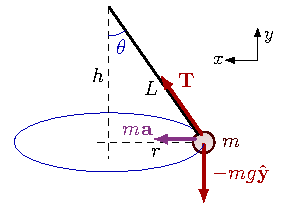
\includegraphics{src/pendulumconical/image1.pdf}
  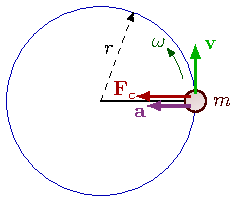
\includegraphics{src/pendulumconical/image2.pdf}
  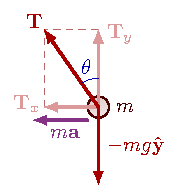
\includegraphics{src/pendulumconical/image3.pdf}
  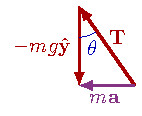
\includegraphics{src/pendulumconical/image4.pdf}
\end{figure}
\newpage
\hrulefill
\section{Lavoro ed energia}
\rule{\linewidth/2}{0.5pt}
\subsection{Quantità di moto}
\subsubsection{Quantità di moto}
La \textbf{quantità di moto} di un punto materiale è il vettore
\begin{equation}
  \boxed{\vec{p} = m \cdot \vec{v}}
\end{equation}
\begin{equation*}
  \left[kg \cdot \frac{m}{s}\right]
\end{equation*}
Se la massa è costante la Seconda Legge di Newton si può scrivere come
\begin{equation*}
  \vec{F} = m \cdot \vec{a} =  m \cdot \frac{d\vec{v}}{dt} = \frac{d m \cdot \vec{v}}{dt} = \frac{d\vec{p}}{dt}
\end{equation*}
\begin{equation}
  \boxed{\vec{F} = \frac{d\vec{p}}{dt}}
\end{equation}

\subsection{Impulso}
\subsubsection{Impulso}
Considerando che l’azione di una forza si svolge nel tempo, definiamo \textbf{impulso della forza} l’integrale della forza nel tempo:
\begin{equation}
  \boxed{\vec{J} = \int_{t_0}^{t_1} \vec{F} \cdot dt}
\end{equation}
\begin{equation*}
  \left[kg \cdot \frac{m}{s}\right]
\end{equation*}
\begin{figure}[H]
  \centering
  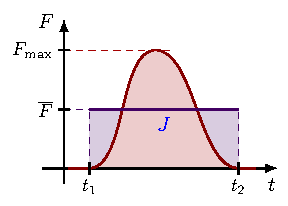
\includegraphics{src/impulse/image1.pdf}
  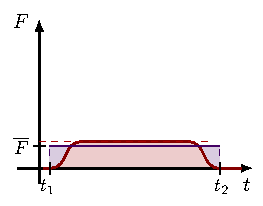
\includegraphics{src/impulse/image2.pdf}
  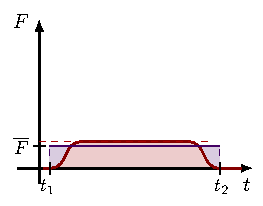
\includegraphics{src/impulse/image3.pdf}
\end{figure}
\subsubsection{Teorema dell’impulso}
\begin{equation}
  \boxed{\vec{J} = \int_{t_0}^{t_1} \vec{F} \cdot dt = \int_{t_0}^{t_1} \frac{d\vec{p}}{dt} \cdot dt = \int_{t_0}^{t_1} d\vec{p} = \vec{p_1} - \vec{p_0} = \Delta \vec{p}}
\end{equation}
Se la massa è costante
\begin{equation}
  \Delta \vec{p} = m \cdot \vec{v_1} - m \cdot \vec{v_0} = m \cdot(\vec{v_1} - \vec{v_0} ) = m \cdot \Delta \vec{v}
\end{equation}
\subsubsection{Teorema di conservazione della quantità di moto}
Se su un punto materiale non agiscono forze, o se la loro risultante è nulla, la quantità di moto si conserva
\begin{equation}
  \boxed{\vec{p_1} + \vec{p_2} = \vec{p_1'} + \vec{p_2'}}
\end{equation}

\subsubsection{Valor medio della Forza agente}
\begin{equation}
  \boxed{\overline{F_m} = \frac{\Delta \vec{p}}{\Delta t}}
\end{equation}

\subsection{Lavoro}
\subsubsection{Lavoro}
Il lavoro è definito come il prodotto scalare tra la forza e lo spostamento
\begin{equation}
  \boxed{W = \vec{F} \cdot \vec{s} = F \cdot s \cdot \cos{\theta}}
\end{equation}
\begin{figure}[H]
  \centering
  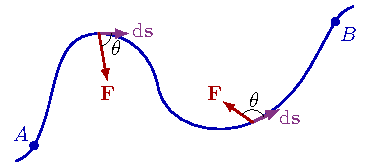
\includegraphics{src/work/image1.pdf}
\end{figure}
\subsubsection{Lavoro di una forza variabile}
Un punto materiale P che sotto l’azione di una forza variabile $\vec{F}$ si muove lungo una traiettoria qualunque tra due punti A e B.
Durante lo spostamento infinitesimo $d\vec{s}$, la forza compie un lavoro infinitesimo:
\begin{equation}
  \boxed{dW = \vec{F} \cdot d\vec{s}}
\end{equation}
Il lavoro totale W compiuto dalla forza da A a B si otterrà sommando il lavoro compiuto lungo
tratti infinitesimi di spostamento:
\begin{equation}
  \boxed{W = \int_{A}^{B} \vec{F} \cdot d\vec{s}}
\end{equation}
Nota che si tratta di una forza e spostamento sono vettori, mentre il lavoro è uno scalare; nell’integrando compare un prodotto scalare.
\begin{equation*}
  W = \int_{A}^{B} (F_x\ dx) + (F_y\ dy) + (F_z\ dz) = \int_{A}^{B} F_x\ dx + \int_{A}^{B} F_y\ dy + \int_{A}^{B} F_z\ dz
\end{equation*}
\begin{equation*}
  W = F_x \int_{A}^{B} dx + F_y \int_{A}^{B} dy + F_z \int_{A}^{B} dz
\end{equation*}
\begin{equation*}
  \left[J = N \cdot m = kg \cdot \frac{m^2}{s^2}\right]
\end{equation*}
\begin{figure}[H]
  \centering
  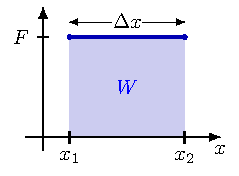
\includegraphics{src/work/image7.pdf}
  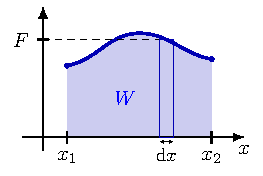
\includegraphics{src/work/image8.pdf}
\end{figure}
\subsubsection{Significato fisico del lavoro}
Il lavoro è una forma di energia.\\
Il risultato del lavoro è un cambiamento della quantità di energia immagazzinata dal sistema.\\
Si distinguono 3 casi:
\begin{align*}
   & \theta < \frac{\pi}{2} \quad dW > 0 \text{ lavoro motore, viene trasferita energia al sistema}    & 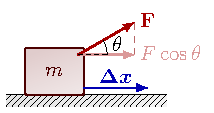
\includegraphics{src/work/image4.pdf} \\
   & \theta = \frac{\pi}{2} \quad dW = 0 \text{ lavoro nullo}                                          & 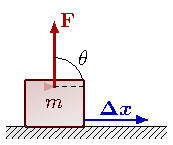
\includegraphics{src/work/image2.pdf} \\
   & \theta > \frac{\pi}{2} \quad dW < 0 \text{ lavoro resistente, viene sottratta energia al sistema} & 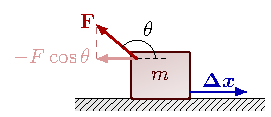
\includegraphics{src/work/image5.pdf}
\end{align*}

\subsubsection{Lavoro della forza peso}
\begin{equation}
  \boxed{W_p = \vec{F_p} \cdot \vec{s} = m \cdot \vec{g} \cdot \vec{s} = mgs \ \cos{\theta} = mgh_1 - mgh_0}
\end{equation}
Il lavoro della forza peso è indipendente dalla traiettoria seguita dal punto materiale, ma dipende solo dalla differenza di quota tra i punti A e B, cioè la direzione in cui si esercita la forza peso.

\subsubsection{Lavoro della forza elastica}
\begin{equation}
  \boxed{W_e = -\frac{1}{2} \cdot k(x_1^2 - x_0^2)}
\end{equation}
Il lavoro della forza elastica è indipendente dalla traiettoria seguita dal punto materiale, ma dipende solo dalla differenza di quota tra i punti A e B, cioè la direzione in cui si esercita la forza elastica.

\subsubsection{Lavoro della forza di attrito}
\begin{equation}
  \boxed{W_a = -\mu \cdot N \cdot s = -\mu \cdot m \cdot g \cdot s \cdot \cos{\theta} = -\mu\ g\ \cos{\theta} ( x_1 - x_0)}
\end{equation}
Il lavoro della forza di attrito è \textbf{dipendente} dal percorso effettivo

\subsection{Potenza}
\subsubsection{Potenza}
La potenza è definita come il rapporto tra il lavoro svolto e il tempo impiegato per svolgerlo
\begin{equation}
  \boxed{P = \frac{dW}{dt}}
\end{equation}


\subsection{Energia}
\subsubsection{Teorema delle forze vive}
Il lavoro è connesso alla variazione di energia cinetica del punto materiale.
\begin{equation}
  \boxed{W_{A \rightarrow B} = \Delta E_c = E_{c\ finale} - E_{c\ iniziale}}
\end{equation}

\begin{equation*}
  W = \int_{A}^{B} \vec{F} \cdot d\vec{s} = \int_{A}^{B} m \cdot \vec{a} \cdot d\vec{s} = \int_{A}^{B} m \cdot \frac{d\vec{v}}{dt} \cdot d\vec{s} = \int_{A}^{B} m \cdot \vec{v} \cdot dt
\end{equation*}

\begin{equation*}
  W = \Delta E_c = \frac{1}{2} \cdot m \cdot v_B^2 - \frac{1}{2} \cdot m \cdot v_A^2 = \frac{1}{2} \cdot m \cdot (v_B^2 - v_A^2) = \frac{1}{2} \cdot m \cdot \Delta v^2
\end{equation*}

\subsubsection{Energia cinetica}
\begin{equation}
  \boxed{E_c = \frac{1}{2} \cdot m \cdot v^2}
\end{equation}

\subsection{Energia potenziale}

\subsubsection{Forze conservative}
Si dicono \textbf{forze conservative} quelle forze il cui lavoro su un punto materiale dipende solo dalle posizioni iniziale e finale e non dal percorso seguito.\\
\begin{align*}
   & \text{Forza peso} \quad \vec{F_p} = m \cdot \vec{g}      \\
   & \text{Forza elastica} \quad \vec{F_e} = -k \cdot \vec{x} \\
\end{align*}
Il lavoro di una forza conservativa lungo un percorso chiuso è nullo
\begin{figure}[H]
  \centering
  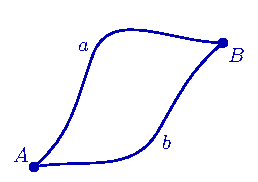
\includegraphics{src/work/image9.pdf}
  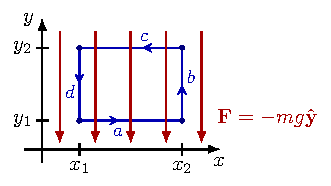
\includegraphics{src/work/image10.pdf}
  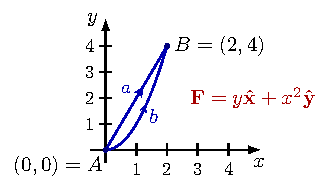
\includegraphics{src/work/image11.pdf}
\end{figure}
\begin{equation}
  \boxed{\oint \vec{F} \cdot d\vec{s} = 0}
\end{equation}
Nota : $\oint$ è l'integrale di linea chiusa, si chiama anche integrale di circuitazione.

\subsubsection{Forze non conservative}
Forze il cui lavoro dipende dal percorso si dicono \textbf{non conservative} o dissipative.
\begin{align*}
   & \text{Forza di attrito} \quad \vec{F_a} = -\mu \cdot \vec{N} \\
   & \text{Forza viscosa} \quad \vec{F_v} = -\eta \cdot \vec{v}
\end{align*}
\subsubsection{Energia potenziale}
Se una forza è conservativa, esiste una funzione scalare $U(\vec{r})$, definita \textbf{energia potenziale}
\begin{equation}
  \boxed{U_P - U_O = - W_{OP} = -\int_{O}^{P} \vec{F} \cdot d\vec{s}}
\end{equation}
dove $O$ è un punto scelto come riferimento(conviene che sia $O$ tale per cui $U_O=0$) e $P$ il punto in questione.
Il significato di questa scelta è il seguente: mentre la forza compie lavoro sul sistema ($W>0$), l’energia potenziale si riduce e si trasforma in energia cinetica, che aumenta.
\subsubsection{Energia potenziale gravitazionale}
\begin{equation}
  \boxed{U_g = mgh}
\end{equation}
\subsubsection{Energia potenziale elastica}
\begin{equation}
  \boxed{U_e = \frac{1}{2}kx^2}
\end{equation}
\subsubsection{Energia meccanica}
\begin{equation}
  \boxed{E_m = E_c + U = \frac{1}{2}  m  v^2 + U = costante}
\end{equation}
\subsubsection{Conservazione dell'energia meccanica}
In presenza di forze conservative, l’energia meccanica si conserva
\begin{equation}
  \boxed{E_m = E_c + U = \frac{1}{2} m v^2 + U = costante}
\end{equation}
\begin{equation*}
  \Delta E_m = E_{c\ finale} - E_{c\ iniziale} + U_{finale} - U_{iniziale} = 0
\end{equation*}
In presenza di forze non conservative, la variazione di energia meccanica tra
stato finale e iniziale coincide con il lavoro delle forze non conservative $W_{nc}$:
\begin{equation}
  \boxed{\Delta E_m = W_{nc} = \int_{A}^{B} \vec{F_{nc}} \cdot d\vec{s}}
\end{equation}
\subsection{Formule utili}
Quantità di moto
\begin{equation*}
  \boxed{\vec{p} = m\vec{v}}
\end{equation*}
Impulso
\begin{equation*}
  \boxed{\vec{J} = \int_{t_0}^{t_1} \vec{F}dt = \Delta \vec{p}}
\end{equation*}
Lavoro
\begin{equation*}
  \boxed{W_{A \rightarrow B} = \int_{A}^{B} \vec{F} \cdot d\vec{s} = F s \cos{\theta}}
\end{equation*}
Potenza
\begin{equation*}
  \boxed{P = \frac{dW}{dt}}
\end{equation*}
se $F$ è costante
\begin{equation*}
  \boxed{P = F \cdot \frac{ds}{dt} =  F \cdot v} \text{ (viene da es.3 tut 14/11/2023)}
\end{equation*}
Lavoro connesso a variazione di energia cinetica
\begin{equation*}
  \boxed{W_{A\rightarrow B} = \Delta E_c = \frac{1}{2} m v_B^2 - \frac{1}{2}  m v_A^2}
\end{equation*}
Energia cinetica
\begin{equation*}
  \boxed{E_c = \frac{1}{2} m v^2}
\end{equation*}
Energia potenziale gravitazionale
\begin{equation*}
  \boxed{U_p = m g  h}
\end{equation*}
Energia potenziale elastica
\begin{equation*}
  \boxed{U_{el} = \frac{1}{2}  k  x^2}
\end{equation*}
Principio di conservazione dell’energia meccanica in presenza solo di forze conservative
\begin{equation*}
  \boxed{E_m = E_c + U = \frac{1}{2} m v^2 + U = costante}
\end{equation*}
se ci sono forze non conservative
\begin{equation*}
  \boxed{\Delta E_m = W_{nc} = \int_{A}^{B} \vec{F_{nc}} \cdot d\vec{s}}
\end{equation*}


\newpage
\hrulefill
\section{Moti relativi}
\rule{\linewidth/2}{0.5pt}
\subsection{Sistemi di riferimento}
\subsubsection{Sistemi di riferimento inerziali}
Un sistema di riferimento è detto \textbf{inerziale} se un punto materiale su cui non agiscono forze esterne è in quiete o in moto rettilineo uniforme.\\
In esso valgono le leggi di Newton.\\
\begin{figure}[H]
  \centering
  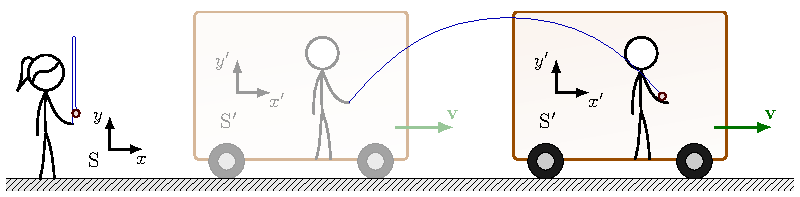
\includegraphics{src/inertialreferenceframe/image1.pdf}
\end{figure}
\subsubsection{Sistemi di riferimento non inerziali}
Un sistema di riferimento è detto \textbf{non inerziale} se in moto accelerato rispetto ad un sistema di riferimento inerziale.\\
In essi si manifestano \textbf{forze apparenti} dette forze di inerzia.

\begin{figure}[H]
  \centering
  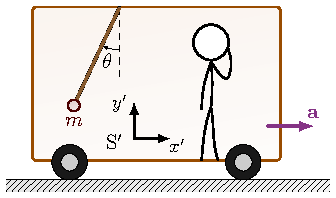
\includegraphics{src/noninertialreferenceframe/image1.pdf}
  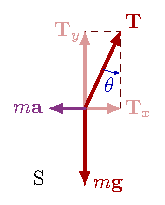
\includegraphics{src/noninertialreferenceframe/image2.pdf}
  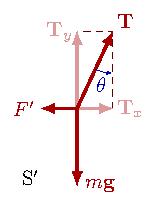
\includegraphics{src/noninertialreferenceframe/image3.pdf}
\end{figure}

\subsubsection{Trasfomazioni di Galileo}
Presi due sistemi di riferimento inerziali $S$ e $S'$, in moto relativo di traslazione uniforme rispetto a $S$ con velocità $\vec{v}$, le coordinate di un punto materiale $P$ in $S$ e $S'$ sono legate dalle \textbf{trasformazioni di Galileo}
\begin{equation}
  \boxed{
    \text{Coordinate}
    \begin{cases}
      x' = x - vt \\
      y' = y      \\
      z' = z      \\
      t' = t
    \end{cases}
    \text{Velocità}
    \begin{cases}
      v_x' = v_x - v \\
      v_y' = v_y     \\
      v_z' = v_z     \\
      t' = t
    \end{cases}
    \text{Accelerazione}
    \begin{cases}
      a_x' = a_x \\
      a_y' = a_y \\
      a_z' = a_z \\
      t' = t
    \end{cases}
  }
\end{equation}
\begin{figure}[H]
  \centering
  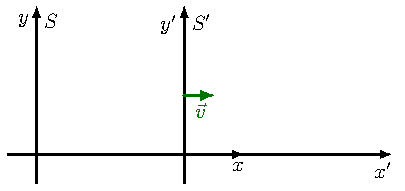
\includegraphics{src/galileo/image1.pdf}
\end{figure}
\subsection{Rototraslazioni}
Presi due sistemi di riferimento inerziali $S$ e $S'$, in moto relativo di rototraslazione uniforme rispetto a $S$ con velocità $\vec{v}$ e accelerazione $\vec{a}$, le coordinate di un punto materiale $P$ in $S$ e $S'$ sono legate dalle \textbf{rototraslazioni}
\begin{figure}[H]
  \centering
  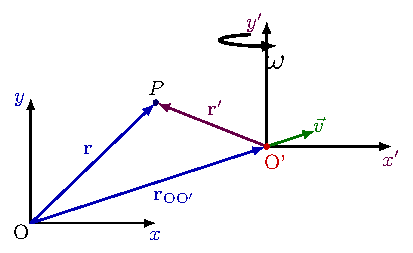
\includegraphics{src/galileo/image2.pdf}
\end{figure}
Si ricava da
\begin{align*}
   & \vec{r} = (x_r,y_r,z_r) = x\hat{i} + y\hat{j} + z\hat{k}                 \\
   & \vec{r'} = (x_{r}',z_{r}',y_{r}') = x'\hat{i} + y'\hat{j} + z'\hat{k}    \\
   & \vec{r_O} = \vec{OO'} = x_{O'} \hat{i} + y_{O'} \hat{j} + z_{O'} \hat{k} \\
   & \vec{r} = \vec{r'} + \vec{r_O}
\end{align*}
\subsection{Teorema delle velocità relative}
La velocità rispetto s $S$ è
\begin{align*}
  \vec{v}(t) & =  \frac{d \vec{r}}{dt}                                                                                                        \\
             & =  \frac{d \vec{r}}{dt} = \textcolor{red}{\frac{d \vec{r_O}}{dt}} + \textcolor{blue}{\frac{d \vec{r'}}{dt}}                    \\
             & \quad \quad \quad = \textcolor{red}{\frac{d \vec{r_O}}{dt} = \vec{v_O}}                                                        \\
             & \quad \quad \quad = \textcolor{blue}{\frac{d \vec{r'}}{dt} = \vec{v'} + \vec{\omega} \times \vec{r'}}\ \text{\footnotemark[1]}
\end{align*}
\footnotetext[1]{Poisson formula $\displaystyle\frac{d\hat{u}}{dt} = \vec{\omega} \times \hat{u}$}
\begin{equation*}
  \vec{v} =  \textcolor{red}{\vec{v_O}} + \textcolor{blue}{\vec{v'} + \vec{\omega} \times \vec{r'}}
\end{equation*}
\begin{equation}
  \boxed{\vec{v} =  \vec{v_O} + \vec{v'} + \vec{\omega} \times \vec{r'}}
\end{equation}
per gli es è più comodo averla come
\begin{equation}
  \boxed{\vec{v} = \vec{v'} + \vec{v_O} + \vec{\omega} \times \vec{r'}}
\end{equation}
\begin{align*}
   & \vec{v}      \quad : \text{ è la velocità del punto P rispetto al sistema } S                      \\
   & \vec{v'}     \quad : \text{ è la velocità del punto P rispetto al sistema } S'                     \\
   & \vec{v_O}    \quad : \text{ è la velocità del sistema } S' \text{ rispetto al sistema } S          \\
   & \vec{\omega} \quad : \text{ è la velocità angolare del sistema } S' \text{ rispetto al sistema } S \\
   & \vec{r'}     \quad : \text{ è il vettore posizione del punto P rispetto al sistema } S'
\end{align*}
\subsubsection{Velocità di trascinamento}
\'E la velocità che il punto mobile P avrebbe se, nell'istante considerato, fosse solidale con il sistema relativo $S'$.
\begin{equation*}
  \vec{v} = \vec{v'} + \underline{\vec{v_O} + \vec{\omega} \times \vec{r'}}
\end{equation*}
\begin{equation}
  \boxed{\vec{v_T} = \vec{v_O} + \vec{w} \times \vec{r'}}
\end{equation}
\newpage
\subsection{Teorema delle accelerazioni relative}
Si dimostra nello stesso modo del teorema delle velocità relative
\begin{equation*}
  \vec{v} = \vec{v_O} + \vec{v'}  + \vec{\omega } \times \vec{r'}
\end{equation*}
\begin{align*}
  \vec{a}(t) & = \frac{d \vec{v}}{dt}                                                                                                                                                                                                                                                                                                \\
             & = \frac{d \vec{v}}{dt} = \textcolor{red}{\frac{d \vec{v_O}}{dt}} + \textcolor{blue}{\frac{d \vec{v'}}{dt}} + \textcolor{violet}{\frac{d (\vec{\omega} \times \vec{r'})}{dt}}                                                                                                                                          \\
             & \quad \quad \quad = \textcolor{red}{\frac{d \vec{v_O}}{dt} = \vec{a_O}}                                                                                                                                                                                                                                               \\
             & \quad \quad \quad = \textcolor{blue}{\frac{d \vec{v'}}{dt} = \vec{a'} + \vec{\omega} \times \vec{v'} = \vec{a'} + \vec{\alpha} \times \vec{r'}}                                                                                                                                                                       \\
             & \quad \quad \quad = \textcolor{violet}{\frac{d (\vec{\omega} \times \vec{r'})}{dt} = \frac{d\vec{\omega}}{dt} \times \vec{r'} + \vec{\omega} \times \underline{\frac{d\vec{r'}}{dt}}} \ \text{\footnotemark[2]}                                                                                                       \\
             & \quad \quad \quad = \textcolor{violet}{ \uuline{\frac{d\vec{\omega}}{dt}} \times \vec{r'} + \vec{\omega} \times \underline{\left( \vec{v'} + \vec{\omega} \times \vec{r'} \right)} = \uuline{\vec{\alpha}} \times \vec{r'} + \vec{\omega} \times \vec{v'} + \omega \times \left(\vec{\omega} \times \vec{r'} \right)} \\
             & = \textcolor{red}{\vec{a_O}}  + \textcolor{blue}{\vec{a'} + \uuline{\vec{\omega} \times \vec{v'}}} + \textcolor{violet}{\vec{\alpha} \times \vec{r'} + \uuline{\vec{\omega} \times \vec{v'}} + \omega \times \left(\vec{\omega} \times \vec{r'} \right) }                                                             \\
             & = \vec{a_O} +\vec{a'} + \vec{\alpha} \times \vec{r'} + 2\left(\vec{\omega} \times \vec{v'}\right) + \omega \times \left(\vec{\omega} \times \vec{r'} \right)
\end{align*}
\footnotetext[2]{Da $\displaystyle \frac{d\vec{r}}{dt} = \vec{v'} + \vec{\omega} \times \vec{r'}$ }
\begin{equation}
  \boxed{\vec{a} = \vec{a'} + \left(\vec{a_O} + \vec{\alpha} \times \vec{r'}\right) + \left(2 \vec{\omega} \times \vec{v'}\right) + \vec{\omega} \times \left(\vec{\omega} \times \vec{r'}\right)}
\end{equation}
\begin{equation*}
  \boxed{\vec{a} = \vec{a'} + \vec{a_T} + \vec{a_{cfg}} + \vec{a_{cor}}}
\end{equation*}
dove
\begin{align*}
   & \vec{a}      \quad \text{ è l'accelerazione del punto P rispetto al sistema } S                       & \\
   & \vec{a'}      \quad \text{ è l'accelerazione del punto P rispetto al sistema } S'                     & \\
   & \vec{a_O}     \quad \text{è l'accelerazione del sistema } S' \text{ rispetto al sistema } S           & \\
   & \vec{\alpha}  \quad \text{ è l'accelerazione angolare del sistema } S' \text{ rispetto al sistema } S & \\
   & \vec{\omega}  \quad \text{ è la velocità angolare del sistema } S' \text{ rispetto al sistema } S     & \\
   & \vec{r'}      \quad \text{ è il vettore posizione del punto P rispetto al sistema } S'                & \\
   & \vec{v'}      \quad \text{ è la velocità del punto P rispetto al sistema } S'
\end{align*}
\subsubsection{Accelerazione di trascinamento}
L'accelerazione di trascinamento è quella accelerazione che il punto mobile P avrebbe se, nell'istante considerato, fosse solidale con il sistema relativo $S'$.
\begin{equation}
  \vec{a} = \vec{a'} + \underline{\vec{a_0} + \vec{\alpha} \times \vec{r'}} + \left(2 \vec{\omega} \times \vec{v'}\right) + \vec{\omega} \times \left(\vec{\omega} \times \vec{r'}\right)
\end{equation}
\begin{equation}
  \boxed{\vec{a_T} = \vec{a_O} + \vec{\alpha} \times \vec{r'}}
\end{equation}
\subsubsection{Accelerazione centrifuga}
L'accelerazione centrifuga è quella accelerazione percepita in un sistema di riferimento rotante, che sembra spingere un oggetto lontano dall'asse di rotazione.\\
Dipende solo da rotazione di $S$' rispetto ad $S$.
\begin{equation*}
  \vec{a} = \vec{a'} + \vec{a_0} + \vec{\alpha} \times \vec{r'} + \left(2 \vec{\omega} \times \vec{v'}\right) + \underline{\vec{\omega} \times \left(\vec{\omega} \times \vec{r'}\right)}
\end{equation*}
\begin{equation}
  \boxed{\vec{a_{cfg}} = \vec{\omega} \times \left(\vec{\omega} \times \vec{r}\right)}
\end{equation}
\begin{figure}[H]
  \centering
  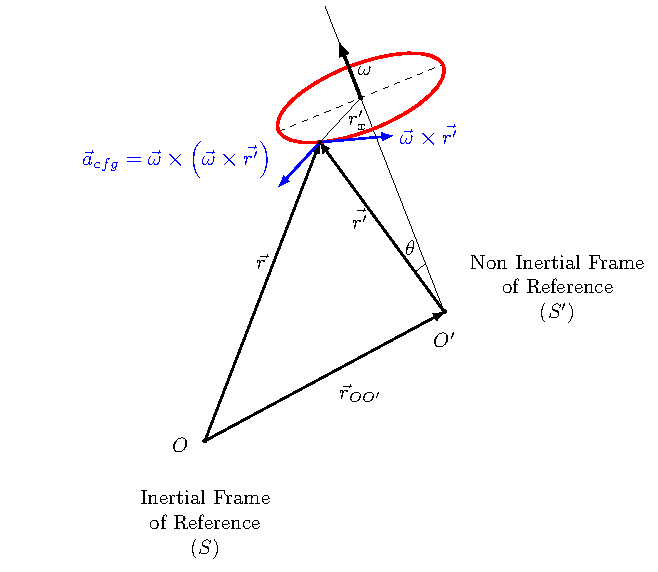
\includegraphics{src/centrifugal/image1.pdf}
\end{figure}
\subsubsection{Accelerazione di Coriolis}
L'accelerazione di Coriolis è l'accelerazione apparente di un punto materiale in un sistema di riferimento rotante, dovuta alla variazione della velocità angolare del sistema di riferimento.\\
Dipende sia dalla rotazione di $S$' rispetto ad $S$ che dalla velocità $\vec{v}$' di $P$ rispetto a $S$'
\begin{equation*}
  \vec{a} = \vec{a'} + \vec{a_0} + \vec{\alpha} \times \vec{r'} + \underline{\left(2 \vec{\omega} \times \vec{v'}\right)} + \vec{\omega} \times \left(\vec{\omega} \times \vec{r'}\right)
\end{equation*}
\begin{equation}
  \boxed{\vec{a_{cor}} = 2\left(\vec{\omega} \times \vec{v}'\right)}
\end{equation}
\begin{figure}[H]
  \centering
  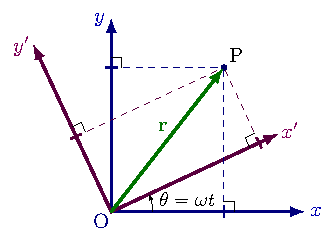
\includegraphics{src/coriolis/image1.pdf}
  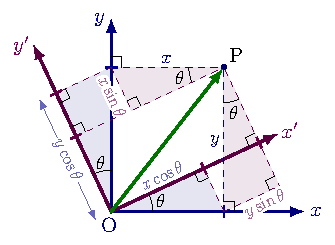
\includegraphics{src/coriolis/image2.pdf}
\end{figure}
\begin{figure}[H]
  \centering
  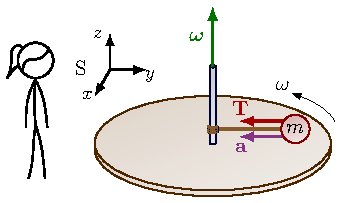
\includegraphics{src/coriolis/image3.pdf}
  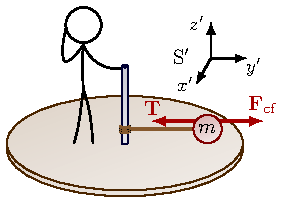
\includegraphics{src/coriolis/image4.pdf}
\end{figure}
\begin{figure}[H]
  \centering
  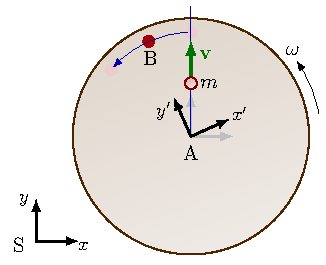
\includegraphics{src/coriolis/image5.pdf}
  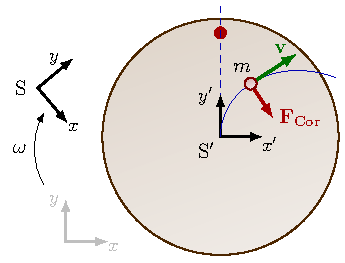
\includegraphics{src/coriolis/image6.pdf}
\end{figure}
\begin{figure}[H]
  \centering
  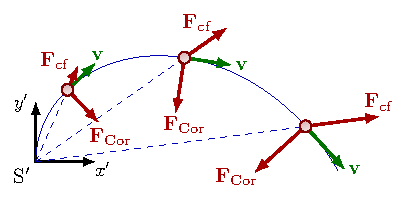
\includegraphics{src/coriolis/image7.pdf}
\end{figure}
\begin{figure}[H]
  \centering
  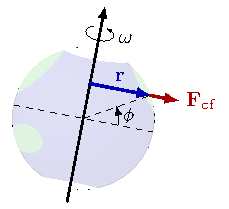
\includegraphics{src/coriolis/image8.pdf}
  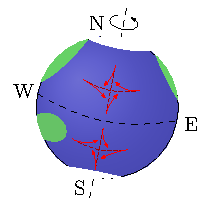
\includegraphics{src/coriolis/image9.pdf}
\end{figure}
\subsection{Forze apparenti}
\begin{equation}
  \boxed{\vec{F'} = m \cdot \vec{a'} = m \cdot \left( \vec{a_T} + \vec{a_{cfg}}+ \vec{a_{cor}}\right)}
\end{equation}
\subsection{Formule utili}
trasformazioni di Galileo
\begin{equation*}
  \boxed{
    \text{Coordinate}
    \begin{cases}
      x' = x - vt \\
      y' = y      \\
      z' = z      \\
      t' = t
    \end{cases}
    \text{Velocità}
    \begin{cases}
      v_x' = v_x - v \\
      v_y' = v_y     \\
      v_z' = v_z     \\
      t' = t
    \end{cases}
    \text{Accelerazione}
    \begin{cases}
      a_x' = a_x \\
      a_y' = a_y \\
      a_z' = a_z \\
      t' = t
    \end{cases}
  }
\end{equation*}
Teorema delle velocità relative
\begin{equation*}
  \boxed{\vec{v} = \vec{v'} + \vec{v_O} + \vec{\omega} \times \vec{r'}}
\end{equation*}
\begin{equation*}
  \boxed{\vec{v} = \vec{v'} + v_{T}}
\end{equation*}
Teorema delle accelerazioni relative
\begin{equation*}
  \boxed{\vec{a} = \vec{a'} + \left(\vec{a_O} + \vec{\alpha} \times \vec{r'}\right) + \left(2 \vec{\omega} \times \vec{v'}\right) + \vec{\omega} \times \left(\vec{\omega} \times \vec{r'}\right)}
\end{equation*}
\begin{equation*}
  \boxed{\vec{a} = \vec{a'} + \vec{a_T} + \vec{a_{cfg}} + \vec{a_{cor}}}
\end{equation*}

\hrulefill
\newpage

\section{Dinamica dei sistemi di punti materiali}
\rule{\linewidth/2}{0.5pt}
\subsection{Sistemi di punti materiali}
\subsubsection{Sistema di punti materiali}
Un sistema di $N$ punti materiali, indicati con $i = (1,...,N)$ di massa $(m_i)$, e individuati da $\vec{(r_i)}$ è un insieme di punti materiali che interagiscono tra loro.\\
\begin{align*}
   & M = \sum_{i=1}^{N} m_i \quad \text{massa totale}                                                                                 \\
   & \vec{P} = \sum_{i=1}^{N} m_i \vec{v_i} \quad \text{quantità di moto totale}                                                      \\
   & \vec{F} = \sum_{i=1}^{N} \vec{F_i} = \sum_{i=1}^{N} \left(\vec{F_i}^{(ext)} + \vec{F_i}^{(int)}\right) \quad \text{forza totale} \\
\end{align*}
Per la Terza Legge di Newton (Principio di azione e reazione) si ha che
\begin{align*}
   & \vec{F_{ij}} = - \vec{F_{ji}} \implies \vec{F_{i}^{(int)}} = 0 \quad \text{forze interne}                                                                                    \\
   & \vec{F} = \sum_{i=1}^{N} \vec{F_i} = \sum_{i=1}^{N} \left(\vec{F_i}^{(ext)} + \cancel{\vec{F_i}^{(int)}}\right) = \sum_{i=1}^{N} \vec{F_i}^{(ext)} \quad \text{forza totale}
\end{align*}
La forza totale agente su un sistema di punti materiali si riduce alla risultante delle sole forze esterne agenti sul sistema perché le forze interne si bilanciano a due a due.\\
Un sistema si dice \textbf{isolato} se la risultante delle forze esterne  è nulla.
\begin{equation*}
  \vec{F}^{(ext)} = 0 \implies \vec{F} = 0 \implies \vec{P} = costante
\end{equation*}
\subsubsection{Principio di conservazione della quantità di moto per un sistema di punti materiali isolato}
Dalla definizione di quantità di moto
\begin{equation*}
  \vec{p} = m\vec{v}
\end{equation*}
\begin{equation*}
  \frac{\vec{p}}{dt} = m\frac{d \vec{v}}{dt}
\end{equation*}
\begin{equation*}
  \frac{d \vec{P}}{dt} = \frac{d}{dt} \sum_{i=1}^{N} m_i \vec{v_i}
\end{equation*}
\begin{equation*}
  \frac{d \vec{P}}{dt} = \sum_{i=1}^{N} m_i \frac{d \vec{v_i}}{dt}
\end{equation*}
\begin{equation*}
  \frac{d \vec{P}}{dt} = \sum_{i=1}^{N} m_i \vec{a_i}
\end{equation*}
\begin{equation*}
  \frac{d \vec{P}}{dt} = \sum_{i=1}^{N} \vec{F_i}
\end{equation*}
\begin{equation*}
  \frac{d \vec{P}}{dt} = \sum_{i=1}^{N} \vec{F_i}^{(ext)} = 0 \quad \text{per un sistema isolato}
\end{equation*}
\begin{equation}
  \boxed{\frac{d \vec{P}}{dt} = 0 \implies \vec{P} = costante}
\end{equation}
\subsection{Centro di massa}
Il centro di massa di un sistema di punti materiali è il punto materiale che si comporta come se tutta la massa del sistema fosse concentrata in esso.\\
\begin{equation}
  \boxed{\vec{r}_{CM} = \frac{1}{m_{tot}} \sum_{i=1}^{N} m_i \vec{r_i}}
\end{equation}
\begin{equation*}
  \begin{cases}
    x_{CM} = \displaystyle \frac{1}{m_{tot}} \sum_{i=1}^{N} m_i x_i \\
    y_{CM} = \displaystyle \frac{1}{m_{tot}} \sum_{i=1}^{N} m_i y_i \\
    z_{CM} = \displaystyle \frac{1}{m_{tot}} \sum_{i=1}^{N} m_i z_i
  \end{cases}
\end{equation*}
\begin{figure}[H]
  \centering
  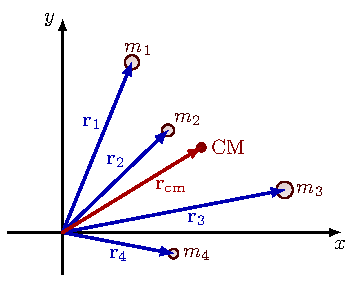
\includegraphics{src/centerofmass/image1.pdf}
  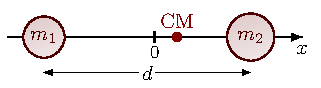
\includegraphics{src/centerofmass/image5.pdf}
\end{figure}
\subsubsection{Centro di massa per sistemi continui}
Solitamente un corpo non ha una densità uniforme, noi in questo caso idealizziamo e possiamo dire che in ogni punto del corpo la densità è costante.\\
\begin{equation*}
  \rho = \frac{m}{V}
\end{equation*}
\begin{equation*}
  \rho = \frac{dm}{dV}
\end{equation*}
\begin{equation*}
  dm = \rho dV
\end{equation*}
Applicando la definizione di centro di massa
\begin{equation*}
  \vec{r}_{CM} = \frac{1}{m_{tot}} \sum_{i=1}^{N} m_i \vec{r_i}
\end{equation*}
\begin{equation*}
  \vec{r}_{CM} = \frac{1}{m_{tot}} \int_{V} \rho(\vec{r}) \vec{r} dV
\end{equation*}
che si può riscrivere come
\begin{equation}
  \boxed{\vec{r}_{CM} = \frac{1}{m_{tot}} \int_{V} \vec{r} dm}
\end{equation}
oppure
\begin{equation}
  \boxed{\vec{r}_{CM} = \frac{1}{m_{tot}} \int_{M} \vec{r} dm}
\end{equation}
\subsection{Moto del centro di massa}
\subsubsection{Velocità e quantità di moto del centro di massa}
\begin{equation*}
  \vec{v} = \frac{d \vec{s}}{dt}
\end{equation*}
\begin{equation*}
  \vec{v}_{CM} = \frac{d \vec{r}_{CM}}{dt}
\end{equation*}
\begin{equation*}
  \vec{v}_{CM} = \frac{d}{dt} \frac{1}{m_{tot}} \sum_{i=1}^{N} m_i \vec{r_i}
\end{equation*}
\begin{equation*}
  \vec{v}_{CM} = \frac{1}{m_{tot}} \sum_{i=1}^{N} \frac{d}{dt}m_i \vec{r_i}
\end{equation*}
\begin{equation*}
  \vec{v}_{CM} = \frac{1}{m_{tot}} \sum_{i=1}^{N} m_i \frac{d\vec{r_i}}{dt}
\end{equation*}
\begin{equation*}
  \vec{v}_{CM} = \frac{1}{m_{tot}} \sum_{i=1}^{N} m_i \vec{v_i}
\end{equation*}
\begin{equation*}
  \vec{v}_{CM} = \frac{1}{m_{tot}} \sum_{i=1}^{N} \vec{p_i}
\end{equation*}
\begin{equation}
  \boxed{\vec{v}_{CM} = \frac{\vec{P}}{m_{tot}}}
\end{equation}
da cui si ricava anche che
\begin{equation}
  \boxed{\vec{P} = m_{tot} \vec{v}_{CM}}
\end{equation}
\subsubsection{Accelerazione del centro di massa}
\begin{equation*}
  \vec{a} = \frac{d \vec{v}}{dt}
\end{equation*}
i passaggi sono analoghi a quelli fatti per la velocità
\begin{equation}
  \boxed{\vec{a}_{CM} = \frac{\vec{F}}{m_{tot}}}
\end{equation}
\subsubsection{Teorema del centro di massa}
\begin{equation}
  \boxed{\vec{F} = m_{tot} \vec{a}_{CM}}
\end{equation}
\subsubsection{Prima equazione cardinale della dinamica dei sistemi di punti materiali}
\begin{equation}
  \boxed{\vec{F} = \frac{d\vec{P}}{dt}= \begin{cases}
      \vec{F}_x = \displaystyle \frac{dP_x}{dt} \\
      \vec{F}_y = \displaystyle \frac{dP_y}{dt} \\
      \vec{F}_z = \displaystyle \frac{dP_z}{dt}
    \end{cases}}
\end{equation}
Osservazioni importanti:
\begin{itemize}
  \item Il principio di conservazione della quantità di moto vale indipendentemente per le tre componenti cartesiane della forza e della quantità di moto.
  \item Il moto del CM è determinato solo dalle forze esterne
  \item Considerando $E_m$
        \begin{enumerate}
          \item Se le forze esterne sono conservative, $E_m = E_c + U$ si conserva
          \item Se le forze esterne sono non conservative, $\Delta E_m = W_{nc}$, la variazione di energia meccanica coincide con il lavoro delle forze non conservative
        \end{enumerate}
  \item Le forze interne sono comunque responsabili dei moti dei singoli punti materiali che
        compongono il sistema. La struttura interna del sistema può quindi variare, così come
        le quantità di moto ed energie cinetiche dei singoli punti materiali.
  \item Le forze interne possono compiere lavoro!
\end{itemize}

\subsection{Teorema di Koenig per l’energia cinetica del centro di massa}
Si considerano due sistemi di punti materiali $S$ e $S'$, in moto relativo di traslazione rispetto a $S$ con velocità $\vec{v}$.
\begin{equation*}
  E_c = E_c' + E_{c\ CM}
\end{equation*}
\subsection{Formule utili}
In un sistema di punti materiali
\begin{equation*}
  \boxed{\vec{P} = \sum_{i=1}^{N} m_i \vec{v_i} \quad m_{tot} = \sum_{i=1}^{N} m_i}
\end{equation*}
Sistema isolato di punti materiali
\begin{equation*}
  \boxed{\vec{F} = \sum_{i=1}^{N} \vec{F_i} = \sum_{i=1}^{N} \left(\vec{F_i}^{(ext)} + \cancel{\vec{F_i}^{(int)}}\right) = \sum_{i=1}^{N} \vec{F_i}^{(ext)} = 0 \implies \vec{P} = costante \implies \frac{d \vec{P}}{dt} = 0}
\end{equation*}
\begin{equation*}
  \boxed{\vec{P} = \sum_{i=1}^{N} m_i \vec{v_i}}
\end{equation*}
Centro di massa\\
punti materiali
\begin{equation*}
  \boxed{\vec{r}_{CM} = \frac{1}{m_{tot}} \sum_{i=1}^{N} m_i \vec{r_i}}
\end{equation*}
corpi continui non uniformi
\begin{equation*}
  \boxed{\vec{r}_{CM} = \frac{1}{m_{tot}} \int_{V} \rho(\vec{r})\ \vec{r}\ dm \quad \text{è utile se densità non uniforme} \quad dm = \rho(\vec{r})\ dV}
\end{equation*}
corpi continui uniformi
\begin{equation*}
  \boxed{\vec{r}_{CM} = \frac{1}{m_{tot}} \int_{V} \vec{r} dm}
\end{equation*}
velocità del centro di massa
\begin{equation*}
  \boxed{\vec{v}_{CM} = \frac{\vec{P}}{m_{tot}}}
\end{equation*}
quantità di moto del centro di massa
\begin{equation*}
  \boxed{\vec{P} = m_{tot} \vec{v}_{CM}}
\end{equation*}
accelerazione del centro di massa
\begin{equation*}
  \boxed{\vec{a}_{CM} = \frac{\vec{F}}{m_{tot}}}
\end{equation*}
forza sul centro di massa
\begin{equation*}
  \boxed{\vec{F} = m_{tot} \vec{a}_{CM}}
\end{equation*}
Teorema di Koenig per l'energia cinetica del centro di massa in moto relativo
\begin{equation*}
  \boxed{E_c = E_c' + E_{c\ CM}}
\end{equation*}
\newpage
\hrulefill
\section{Urti}
\rule{\linewidth/2}{0.5pt}
\subsection{Tipi di urti}
\subsubsection{Urti elastici}
\begin{equation*}
  \begin{cases}
    \text{Conservazione della quantità di moto} \\
    \text{Conservazione dell'energia cinetica}
  \end{cases}
\end{equation*}
\begin{equation*}
  \begin{cases}
    m_1 \vec{v_1} + m_2 \vec{v_2} = m_1 \vec{v_1'} + m_2 \vec{v_2'} \\
    \frac{1}{2} m_1 v_1^2 + \frac{1}{2} m_2 v_2^2 = \frac{1}{2} m_1 v_1'^2 + \frac{1}{2} m_2 v_2'^2
  \end{cases}
\end{equation*}
\begin{equation*}
  v_1' = \frac{(m_1 - m_2)v_1 + (2m_2)v_2}{m_1 + m_2}
\end{equation*}
\begin{equation*}
  v_2' = \frac{(2m_1)v_1 + (m_2 - m_1)v_2}{m_1 + m_2}
\end{equation*}
\begin{figure}[H]
  \centering
  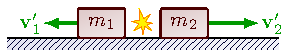
\includegraphics{src/impacts/image2.pdf}
\end{figure}
\subsubsection{Urti anelastici}
\begin{equation*}
  \begin{cases}
    \text{Conservazione della quantità di moto} \\
    \text{Dissipazione dell'energia cinetica}
  \end{cases}
\end{equation*}
\begin{equation*}
  \begin{cases}
    m_1 \vec{v_1} + m_2 \vec{v_2} = (m_1 + m_2) \vec{v'} \\
    \Delta E_c = E_{c\ iniziale} - E_{c\ finale}
  \end{cases}
\end{equation*}
\begin{figure}[H]
  \centering
  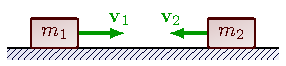
\includegraphics{src/impacts/image1.pdf}
  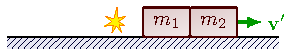
\includegraphics{src/impacts/image3.pdf}
\end{figure}
\subsubsection{Urti completamente anaelastici}
I corpi restano attaccati dopo l'urto
\begin{equation*}
  \begin{cases}
    \text{Conservazione della quantità di moto} \\
  \end{cases}
\end{equation*}
\begin{equation*}
  \begin{cases}
    m_1 \vec{v_1} + m_2 \vec{v_2} = (m_1 + m_2) \vec{v'} \\
  \end{cases}
\end{equation*}
\begin{equation*}
  v' = \frac{m_1 v_1 + m_2 v_2}{m_1 + m_2}
\end{equation*}
\begin{figure}[H]
  \centering
  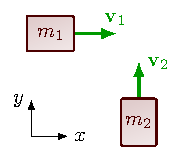
\includegraphics{src/impacts/image4.pdf}
  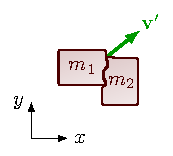
\includegraphics{src/impacts/image5.pdf}
  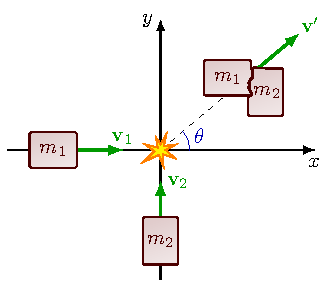
\includegraphics{src/impacts/image6.pdf}
\end{figure}
\subsection{Pendolo balistico}
Si può determinare la velocità iniziale del proiettile considerando che :
\begin{enumerate}
  \item Urto perfettamente anaelastico pendolo-proiettile $\implies m_1(v_{1\ ini}) + m_2(v_{2\ ini}) = (m_1 + m_2) v_{fin}$ \\
  \item Dopo l'urto solo forze conservative $\implies E_{m\ ini} = E_{m\ fin}$
\end{enumerate}
\begin{figure}[H]
  \centering
  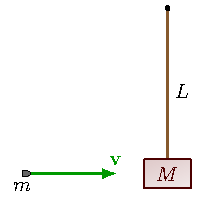
\includegraphics{src/impacts/image7.pdf}
  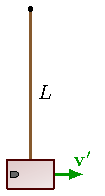
\includegraphics{src/impacts/image8.pdf}
  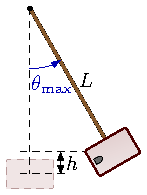
\includegraphics{src/impacts/image9.pdf}
\end{figure}
\subsection{Formule utili}
Urti elastici
\begin{equation*}
  \boxed{
    \begin{cases}
      m_1 \vec{v_1} + m_2 \vec{v_2} = m_1 \vec{v_1'} + m_2 \vec{v_2'} \\
      \frac{1}{2} m_1 v_1^2 + \frac{1}{2} m_2 v_2^2 = \frac{1}{2} m_1 v_1'^2 + \frac{1}{2} m_2 v_2'^2
    \end{cases}
    v_1' = \frac{(m_1 - m_2)v_1 + (2m_2)v_2}{m_1 + m_2}}
\end{equation*}
Urti anelastici
\begin{equation*}
  \boxed{
    \begin{cases}
      m_1 \vec{v_1} + m_2 \vec{v_2} = (m_1 + m_2) \vec{v'} \\
      \Delta E_c = E_{c\ iniziale} - E_{c\ finale} = W_{nc}
    \end{cases}}
\end{equation*}
Urti completamente anaelastici
\begin{equation*}
  \boxed{
    \begin{cases}
      m_1 \vec{v_1} + m_2 \vec{v_2} = (m_1 + m_2) \vec{v'} \\
    \end{cases}
    v' = \frac{m_1 v_1 + m_2 v_2}{m_1 + m_2} \quad \Delta E_m = 0 \quad \text{dopo l'urto}}
\end{equation*}
\newpage
\hrulefill
\section{Momento angolare e momento della forza per punti materiali e sistemi di punti materiali}
\rule{\linewidth/2}{0.5pt}
\subsection{Momenti per punti materiali}
Consideriamo un punto che si muove lungo una traiettoria curvilinea con $\vec{p} = m\vec{v}$.\\
Il suo moto può essere visto come una \textbf{rotazione} rispetto ad un qualche punto fisso che chiamiamo \textbf{polo} (o \textbf{centro di rotazione}) da cui il punto dista $\vec{r}$ ad un dato istante.
\begin{figure}[H]
  \centering
  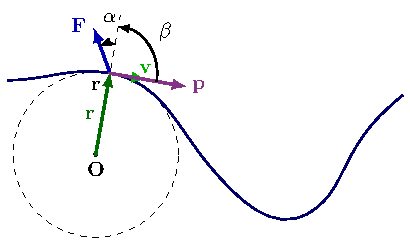
\includegraphics{src/angularmomentum/image3.pdf}
\end{figure}
\subsubsection{Momento angolare per un punto materiale}
\begin{equation}
  \boxed{\vec{L} = \vec{r} \times \vec{p}}
\end{equation}
\begin{equation*}
  \boxed{\vec{L} = r p \sin{\beta}}
\end{equation*}
\begin{equation*}
  \boxed{\vec{L} = \vec{p} h}
\end{equation*}
con $h = \sin{\theta}$ distanza della retta d'azione di $\vec{p}$ dal punto materiale dal polo.
\begin{figure}[H]
  \centering
  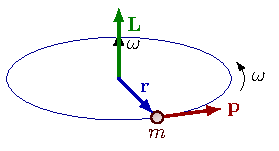
\includegraphics{src/angularmomentum/image1.pdf}
  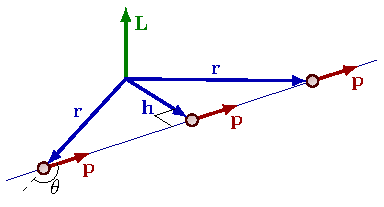
\includegraphics{src/angularmomentum/image2.pdf}
\end{figure}
\subsubsection{Momento della forza per un punto materiale}
\begin{equation}
  \boxed{\vec{M} = \vec{r} \times \vec{F}}
\end{equation}
\begin{equation*}
  \boxed{\vec{M} = r F \sin{\alpha}}
\end{equation*}
\subsubsection{Teorema del momento angolare}
\begin{equation*}
  \frac{d\vec{L}}{dt} = \frac{d(\vec{r} \times \vec{p})}{dt}
\end{equation*}
\begin{equation*}
  \frac{d\vec{L}}{dt} = \frac{d(\vec{r} \times m\vec{v})}{dt}
\end{equation*}
\begin{equation*}
  \frac{d\vec{L}}{dt} = \frac{d\vec{r}}{dt} \times m\vec{v} + \vec{r} \times \frac{d(m\vec{v})}{dt}
\end{equation*}
\begin{equation*}
  \frac{d\vec{L}}{dt} = \cancel{\vec{v} \times m\vec{v}} + \vec{r} \times m\vec{a}
\end{equation*}
\begin{equation*}
  \frac{d\vec{L}}{dt} = \vec{r} \times m\vec{a}
\end{equation*}
\begin{equation*}
  \frac{d\vec{L}}{dt} = \vec{r} \times \vec{F}
\end{equation*}
\begin{equation*}
  \frac{d\vec{L}}{dt} = \vec{M}
\end{equation*}
\begin{equation}
  \boxed{\frac{d\vec{L}}{dt} = \vec{M}}
\end{equation}

\subsubsection{Principio di conservazione del momento angolare}
\begin{equation}
  \boxed{\vec{M} = 0 \implies \frac{d\vec{L}}{dt} = 0 \implies \vec{L} = costante}
\end{equation}
\begin{align*}
  \vec{M} = 0 & \implies \vec{r} \times \vec{F} = 0 \\
              & \implies \vec{F} = 0
\end{align*}
\subsubsection{Teorema momento dell'impulso}
\begin{equation}
  \boxed{ \Delta \vec{L} = \vec{r} \times \vec{J}}
\end{equation}
\begin{equation*}
  \Delta \vec{L} = \vec{r} \times \Delta \vec{p}
\end{equation*}
\subsection{Momenti di sistemi di punti materiali}
\subsubsection{Momento angolare per un sistema di punti materiali}
\begin{equation}
  \boxed{\vec{L} = \sum_{i=1}^{N} \vec{L_i}}
\end{equation}
\begin{equation*}
  \vec{L} = \sum_{i=1}^{N} \vec{r_i} \times \vec{p_i}
\end{equation*}
\begin{equation*}
  \vec{L} = \sum_{i=1}^{N} \vec{r_i} \times m_i \vec{v_i}
\end{equation*}
\subsubsection{Momento della forza per un sistema di punti materiali}
\begin{equation}
  \boxed{\vec{M} = \sum_{i=1}^{N} \vec{M_i}}
\end{equation}
\begin{equation*}
  \vec{M} = \sum_{i=1}^{N} \vec{r_i} \times \vec{F_i}
\end{equation*}

\begin{multicols}{2}
  \noindent
  Si dimostra che come conseguenza del III principio della dinamica, il momento totale di un sistema di punti materiali è dato dalla somma dei soli momenti delle forze esterne applicate.
  \columnbreak
  \noindent
  \\
  Le forze interne non contribuiscono al momento della forza totale.
\end{multicols}
\begin{equation*}
  \vec{M} = \sum_{i=1}^{N} \vec{r_i} \times \vec{F_i}^{(ext)}
\end{equation*}

\subsubsection{Teorema del momento angolare per un sistema di punti materiali}
La \textbf{variazione del momento angolare} $\vec{L}$ di un sistema di punti materiali \textbf{dipende} dal \textbf{momento totale delle forze applicate} $\vec{M}$ e dal \textbf{moto del polo} $\vec{v}_O$ e dal \textbf{moto del CM} $\vec{v}_{CM}$.
\begin{equation}
  \boxed{\frac{d\vec{L}}{dt} = \vec{M} - \vec{v}_O \times m \vec{v}_{CM}}
\end{equation}

\subsubsection{Momento della forza in relazione al lavoro}
\begin{equation*}
  W = \vec{M} \cdot \Delta \vec{\theta}
\end{equation*}
\subsection{Formule utili}
Momento angolare di un punto materiale
\begin{equation*}
  \boxed{\vec{L} = \vec{r} \times \vec{p}}
\end{equation*}
Momento della forza per un punto materiale
\begin{equation*}
  \boxed{\vec{M} = \vec{r} \times \vec{F}}
\end{equation*}
Momento angolare di un sistema di punti materiali
\begin{equation*}
  \boxed{\vec{L} = \sum_{i=1}^{N} \vec{L_i}}
\end{equation*}
Momento della forza per un sistema di punti materiali
\begin{equation*}
  \boxed{\vec{M} = \sum_{i=1}^{N} \vec{M_i}}
\end{equation*}
Teorema del momento angolare
\begin{equation*}
  \boxed{\frac{d\vec{L}}{dt} = \vec{M}}
\end{equation*}
Teorema del momento dell'impulso
\begin{equation*}
  \boxed{ \Delta \vec{L} = \vec{r} \times \vec{J} = \vec{r} \times \Delta \vec{p}}
\end{equation*}
Principio di conservazione del momento angolare, se $L$ è costante $M = 0$
\begin{equation*}
  \boxed{\vec{M} = 0 \implies \frac{d\vec{L}}{dt} = 0 \implies \vec{L} = costante}
\end{equation*}
Teorema del momento angolare per un sistema di punti materiali
\begin{equation*}
  \boxed{\frac{d\vec{L}}{dt} = \vec{M} - \vec{v}_O \times m \vec{v}_{CM}}
\end{equation*}
Momento della forza in relazione al lavoro
\begin{equation*}
  \boxed{W = \vec{M} \cdot \Delta \vec{\theta}}
\end{equation*}
\newpage
\hrulefill
\section{Cinematica del corpo rigido}
\rule{\linewidth/2}{0.5pt}
\subsection{Cinematica del corpo rigido}
Nel caso più generale il moto di un corpo rigido può essere composto da un moto di \textbf{traslazione} del \textbf{centro di massa} e da un \textbf{moto di rotazione} attorno al centro di massa, viene caratterizzato dalle seguenti equazioni\\
\subsubsection{Moto di rototraslazione}
\textbf{Moto di traslazione}\\
Si usa la \textbf{I equazione cardinale della dinamica} per il centro di massa
\begin{equation}
  \boxed{\vec{F}^{(ext)} = \frac{d\vec{P}}{dt} = m_{tot} \vec{a}_{CM}}
\end{equation}
\textbf{Moto di rotazione}\\
Si usa la \textbf{II equazione cardinale della dinamica} per il centro di massa
\begin{equation}
  \boxed{\vec{M}^{(ext)} = \frac{d\vec{L}}{dt}}
\end{equation}
\textbf{Energia in un moto di rototraslazione}\\
Si usa il \textbf{il teorema lavoro-energia} per i sistemi di punti
\begin{equation}
  \boxed{\Delta E_c = W}
\end{equation}
\textbf{Principio di conservazione della quantità di moto}\\
Se un sistema è \textbf{isolato} ($\vec{F}^{(ext)} = 0$)
\begin{equation}
  \boxed{\vec{P}_{tot} = \vec{P}_{CM} = costante}
\end{equation}
\textbf{Principio di conservazione del momento angolare}\\
Se un sistema è ha un momento nullo ($\vec{M}^{(ext)} = 0$)
\begin{equation}
  \boxed{\vec{L}_{tot} = \vec{L}_{CM} = costante}
\end{equation}
\subsection{Equilibrio statico di un corpo rigido}
\subsubsection{Equilibrio statico}
Un corpo rigido è in \textbf{equilibrio statico} se non trasla e non ruota, ovvero
\begin{enumerate}
  \item La risultante delle forze esterne è nulla : $\sum \vec{F}^{(ext)} = 0 \implies \frac{d\vec{P}}{dt} = 0 \implies \vec{P} = costante \implies m_{tot}\ \vec{v}_{CM} = 0 $
  \item Il momento delle forze esterne e interne è nullo : $\sum \vec{M} = 0 \implies \frac{d\vec{L}}{dt}=0$%correggi il concetto se interne e esterne va bene
\end{enumerate}
\subsubsection{Coppia di forze}
Una \textbf{coppia di forze} è una coppia di forze \textbf{uguali} e \textbf{opposte} applicate in punti \textbf{diversi} di un corpo rigido.\\
\begin{enumerate}
  \item La risultante delle forze è nulla : $\sum \vec{F}^{(ext)} = 0 \implies \frac{d\vec{P}}{dt} = 0 \implies \vec{P} = costante \implies m_{tot}\ \vec{v}_{CM} = 0 $
  \item Il momento delle forze \textbf{non è nullo} : $\sum \vec{M} \neq 0 \implies \frac{d\vec{L}}{dt} \neq 0$
\end{enumerate}
\subsubsection{Forze parallele}
Un sistema di forze parallele si può sempre ridurre ad una sola forza risultante applicata ad un punto definito \textbf{centro delle forze parallele} che si trova così:
\begin{equation*}
  \boxed{\vec{r}_C = \displaystyle \frac{\sum F_i \vec{r}_i}{\sum F_i}}
\end{equation*}

\subsubsection{Corpi soggetti a forza peso}
Per i corpi soggetti alla forza peso si può definire il \textbf{baricentro o centro di gravità} come il punto al quale si può pensare applicata la forza peso\\
Si può dimostrare che il \textbf{centro di gravità coincide con il centro di massa del sistema}, seppure concettualmente questi due punti abbiano definizioni distinte.
\begin{equation*}
  \vec{r}_{CG} \equiv \vec{r}_{CM}
\end{equation*}
\begin{equation*}
  \boxed{\vec{r}_{CG} = \frac{1}{m_{tot}} \sum_{i=1}^{N} m_i \vec{r_i}}
\end{equation*}
\begin{figure}[H]
  \centering
  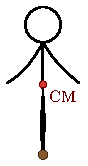
\includegraphics{src/centerofgravity/image1.pdf}
  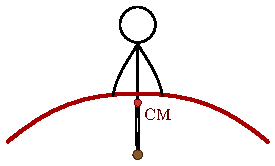
\includegraphics{src/centerofgravity/image2.pdf}
  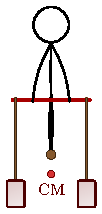
\includegraphics{src/centerofgravity/image3.pdf}
  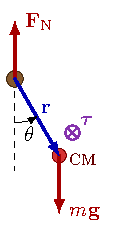
\includegraphics{src/centerofgravity/image4.pdf}
\end{figure}

\subsubsection{Concetto importante}
Un sistema complesso di forze applicate su un corpo rigido può essere semplificato attraverso la decomposizione in due componenti principali:
\begin{itemize}
  \item Una \textbf{forza risultante} \( \mathbf{F} \), che agisce lungo una specifica linea d'azione. Questa forza determina l'effetto traslazionale sul corpo, ovvero il movimento del centro di massa del corpo lungo una traiettoria definita dalla direzione di \( \mathbf{F} \). La forza risultante è scelta in modo tale da avere un momento nullo rispetto a un polo arbitrariamente scelto, facilitando l'analisi del movimento traslazionale senza considerare gli effetti rotazionali.
  \item Una \textbf{coppia di forze}, caratterizzata da due forze parallele, uguali in modulo e opposte in direzione, ma applicate in punti diversi del corpo. La coppia di forze non produce una risultante netta (ovvero, non sposta il centro di massa), ma genera un momento \( \mathbf{M} \) che induce un movimento rotazionale attorno al polo. Il momento generato dalla coppia è significativo perché è indipendente dalla scelta del polo, consentendo un'analisi uniforme degli effetti rotazionali sul corpo.
\end{itemize}

\subsection{Rotazione attorno ad un asse fisso}
\subsubsection{Energia cinetica e momento di inzerzia}
\begin{equation*}
  E_c = \sum_{i=1}^{N} E_i
\end{equation*}
\begin{equation*}
  E_c = \sum_{i=1}^{N} \frac{1}{2} m_i v_i^2
\end{equation*}
pocihé \(v_i = \omega r_i\)
\begin{equation*}
  E_c =  \sum_{i=1}^{N}\frac{1}{2} m_i w^2 r_i^2
\end{equation*}
\begin{equation*}
  E_c = \frac{1}{2} w^2 \sum_{i=1}^{N} m_i r_i^2
\end{equation*}
poiché \(\displaystyle \sum_{i=1}^{N} m_i r_i^2 = I\) momento di inerzia (spiego dopo)
\begin{equation}
  \boxed{E_c = \frac{1}{2} I w^2}
\end{equation}

\subsubsection{Momento di inerzia}
Il \textbf{momento di inerzia} di un corpo rispetto ad un asse è una misura della resistenza del corpo a ruotare attorno a quell'asse.\\
\begin{equation*}
  \boxed{I = \int r^2 dm}
\end{equation*}
Remember that "centro di massa in corpi continui"?
\begin{equation*}
  \rho = \frac{m}{V}
\end{equation*}
\begin{equation*}
  \rho = \frac{dm}{dV}
\end{equation*}
\begin{equation*}
  dm = \rho dV
\end{equation*}
Se la densità è linearmente variabile
\begin{equation*}
  \rho = \rho(\vec{r}) = a \rho_o
\end{equation*}
\begin{equation*}
  dm = \rho(\vec{r}) dV
\end{equation*}
\begin{equation*}
  dm = a \rho_o dV
\end{equation*}
Inoltre la sezione di una sbarretta la trovo come
\begin{equation*}
  dV = A dx
\end{equation*}
\begin{equation*}
  I = \int r^2 dm
\end{equation*}
\begin{equation*}
  I = \int_{0}^{L} r^2 a \rho_o dV
\end{equation*}
\begin{equation*}
  I = a \rho_o \int_{0}^{L} r^2 A dx
\end{equation*}
\begin{equation*}
  I = a \rho_o A \int_{0}^{L} r^2 dx
\end{equation*}
\subsubsection{Momento di inerzia da momento angolare}
\begin{equation}
  \boxed{\vec{L} = I \vec{w}}
\end{equation}
\subsubsection{Teorema di Huygens-Steiner (o teorema degli assi paralleli)}
Il momento d’inerzia \(I\) di un corpo rigido di massa \(m_{tot}\) rispetto ad un asse di rotazione che si trova ad una distanza \(d\) dall’asse ad esso parallelo e passante per il centro di massa del sistema è dato da
\begin{equation}
  \displaystyle \boxed{I = I_{CM} + d^2 m_{tot}}
\end{equation}
\begin{figure}[H]
  \centering
  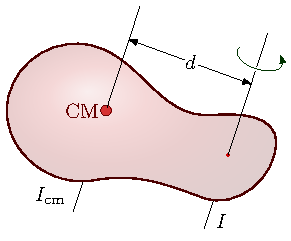
\includegraphics[width=0.2\textwidth]{src/huygens-steiner/image1.pdf}
  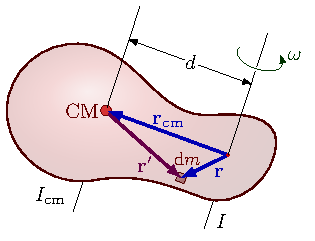
\includegraphics[width=0.2\textwidth]{src/huygens-steiner/image2.pdf}
  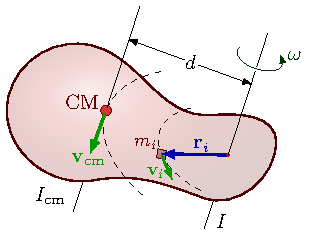
\includegraphics[width=0.2\textwidth]{src/huygens-steiner/image3.pdf}
  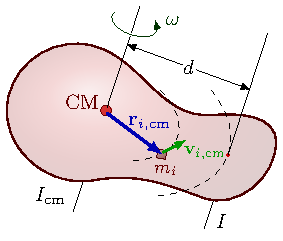
\includegraphics[width=0.2\textwidth]{src/huygens-steiner/image4.pdf}
\end{figure}
\subsection{Momento di inerzia di corpi noti}
\subsubsection{Barretta sottile}
\begin{enumerate}
  \item Omogenea (\(\rho = \) costante) in rotazione per un asse passante per un estremo
        \begin{equation*}
          \rho = \frac{m}{L}
        \end{equation*}
        \begin{equation*}
          \rho = \frac{dm}{dx}
        \end{equation*}
        \begin{equation*}
          dm = \rho dx
        \end{equation*}
        \begin{equation*}
          I = \int r^2 dm
        \end{equation*}
        \begin{equation*}
          I = \int_{0}^{L} r^2 \rho dx
        \end{equation*}
        \begin{equation*}
          I = \int_{0}^{L} r^2 \frac{m}{L} dx
        \end{equation*}
        \begin{equation*}
          I = \frac{m}{L} \int_{0}^{L} r^2 dx
        \end{equation*}
        \begin{equation*}
          I = \frac{m}{L} \int_{0}^{L} x^2 dx
        \end{equation*}
        \begin{equation*}
          I = \frac{m}{L} \left[\frac{x^3}{3}\right]_{0}^{L}
        \end{equation*}
        \begin{equation*}
          I = \frac{m}{L} \frac{L^3}{3}
        \end{equation*}
        \begin{equation*}
          I = \frac{1}{3} m L^2
        \end{equation*}
        \begin{equation*}
          \boxed{I = \frac{1}{3} m L^2}
        \end{equation*}
        \begin{figure}[H]
          \centering
          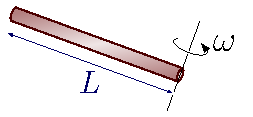
\includegraphics[width=0.2\textwidth]{src/momentofinertia/image1.pdf}
        \end{figure}
  \item Omoegena (\(\rho = \) costante) in rotazione per un asse passante per il centro di massa
        \begin{equation*}
          \rho = \frac{m}{L}
        \end{equation*}
        \begin{equation*}
          \rho = \frac{dm}{dx}
        \end{equation*}
        \begin{equation*}
          dm = \rho dx
        \end{equation*}
        \begin{equation*}
          I = \int r^2 dm
        \end{equation*}
        \begin{equation*}
          I = \int_{0}^{L} r^2 \rho dx
        \end{equation*}
        \begin{equation*}
          I = \int_{0}^{L} r^2 \frac{m}{L} dx
        \end{equation*}
        \begin{equation*}
          I = \frac{m}{L} \int_{-\frac{L}{2}}^{\frac{L}{2}} r^2 dx
        \end{equation*}
        \begin{equation*}
          I = \frac{m}{L} \int_{-\frac{L}{2}}^{\frac{L}{2}} x^2 dx
        \end{equation*}
        \begin{equation*}
          I = \frac{m}{L} \left[\frac{x^3}{3}\right]_{-\frac{L}{2}}^{\frac{L}{2}}
        \end{equation*}
        \begin{equation*}
          I = \frac{m}{L} \frac{L^3}{24}
        \end{equation*}
        \begin{equation*}
          \boxed{I = \frac{1}{12} m L^2}
        \end{equation*}
        \begin{figure}[H]
          \centering
          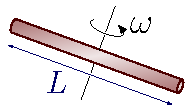
\includegraphics[width=0.2\textwidth]{src/momentofinertia/image2.pdf}
        \end{figure}
  \item Non omogenea (\(\rho = \rho_0 x\)) in rotazione rispetto ad un asse passante per un estremo
        \begin{equation*}
          \rho = \rho_0 x
        \end{equation*}
        \begin{equation*}
          \rho = \frac{dm}{dx}
        \end{equation*}
        \begin{equation*}
          dm = \rho dx
        \end{equation*}
        \begin{equation*}
          dm = \rho_0 x dx
        \end{equation*}
        \begin{equation*}
          I = \int r^2 dm
        \end{equation*}
        \begin{multicols}{2}
          \begin{equation*}
            I = \int_{0}^{L} r^2 \rho dx
          \end{equation*}
          \begin{equation*}
            I = \int_{0}^{L} r^2 \rho_0 x dx
          \end{equation*}
          \begin{equation*}
            I = \rho_0 \int_{0}^{L} r^2 x dx
          \end{equation*}
          \begin{equation*}
            I = \rho_0 \int_{0}^{L} x^3 dx
          \end{equation*}
          \begin{equation*}
            I = \rho_0 \left[\frac{x^4}{4}\right]_{0}^{L}
          \end{equation*}
          \begin{equation*}
            I = \rho_0 \frac{L^4}{4}
          \end{equation*}

          \columnbreak
          \noindent
          \\
          \begin{equation*}
            dm = \rho_0 x dx
          \end{equation*}
          \begin{equation*}
            m = \int \rho dx
          \end{equation*}
          \begin{equation*}
            m_{tot} = \int_{0}^{L} \rho_0 x dx
          \end{equation*}
          \begin{equation*}
            m_{tot} = \rho_0 \int_{0}^{L} x dx
          \end{equation*}
          \begin{equation*}
            m_{tot} = \rho_0 \left[\frac{x^2}{2}\right]_{0}^{L}
          \end{equation*}
          \begin{equation*}
            m_{tot} = \rho_0 \frac{L^2}{2}
          \end{equation*}
          \begin{equation*}
            \rho_0 = \frac{m_{tot}}{\frac{L^2}{2}}
          \end{equation*}
          \begin{equation*}
            \rho_0 = \frac{2 m_{tot}}{L^2}
          \end{equation*}
        \end{multicols}
        \begin{equation*}
          I = \frac{2 m_{tot}}{L^2} \frac{L^4}{4}
        \end{equation*}
        \begin{equation*}
          \boxed{I = \frac{1}{2} m_{tot} L^2}
        \end{equation*}
        \begin{figure}[H]
          \centering
          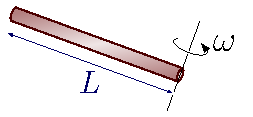
\includegraphics[width=0.2\textwidth]{src/momentofinertia/image1.pdf}
        \end{figure}
\end{enumerate}
\newpage
\subsubsection{Cilindro}
\begin{enumerate}
  \item Pieno omogeneo (\(\rho = \) costante) in rotazione (\textbf{coassiale}) attorno al suo asse
        di simmetria perpendicolare alla base e passante per il suo centro
        \begin{multicols}{2}
          \begin{equation*}
            \rho = \frac{m}{V}
          \end{equation*}
          \begin{equation*}
            \rho = \frac{dm}{dV}
          \end{equation*}
          \columnbreak
          \noindent
          \\
          \begin{equation*}
            V = \pi R^2 h
          \end{equation*}
          \begin{equation*}
            dV = 2 \pi R h dr
          \end{equation*}
        \end{multicols}
        \begin{equation*}
          dm = \rho\ dV
        \end{equation*}
        \begin{equation*}
          dm = \rho\  2 \pi R h\ dr
        \end{equation*}
        \begin{equation*}
          I = \int r^2 dm
        \end{equation*}
        \begin{equation*}
          \boxed{I = \frac{1}{2} m R^2}
        \end{equation*}
        \begin{figure}[H]
          \centering
          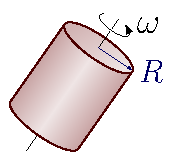
\includegraphics[width=0.2\textwidth]{src/momentofinertia/image3.pdf}
        \end{figure}
  \item Cavo omogeneo (\(\rho = \) costante) in rotazione attorno ad un asse passante per il suo centro e perpendicolare all'altezza
        \begin{equation*}
          \boxed{I = \frac{1}{12} m h^2}
        \end{equation*}
        \begin{figure}[H]
          \centering
          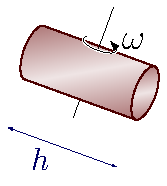
\includegraphics[width=0.2\textwidth]{src/momentofinertia/image4.pdf}
        \end{figure}
  \item Guscio cilindrico cavo, con superficie omogenea (\(\rho = \) costante) , in rotazione (\textbf{coassiale}) attorno al suo asse
        di simmetria perpendicolare alla base e passante per il suo centro
        \begin{equation*}
          \boxed{I = m R^2}
        \end{equation*}
        \begin{figure}[H]
          \centering
          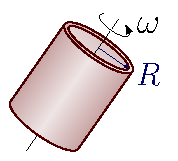
\includegraphics[width=0.2\textwidth]{src/momentofinertia/image5.pdf}
        \end{figure}
\end{enumerate}
\subsubsection{Momento di inerzia di corpi rigidi composti}
Nel caso di corpi rigidi composti, il momento d’inerzia può essere calcolato come somma dei momenti d’inerzia di singole parti/componenti del corpo, facendo attenzione ad individuare correttamente l’asse di rotazione e le distanze da esso.
\subsection{Formule importanti nei moti di rotazione}
Ricordiamo che
\begin{equation*}
  \vec{v} = \vec{\omega} \times \vec{r}
\end{equation*}
\begin{equation*}
  \vec{a} = \vec{\alpha} \times \vec{r} + \vec{\omega} \times (\vec{\omega} \times \vec{r})
\end{equation*}
\begin{equation*}
  \vec{a} = \vec{\alpha} \times \vec{r} + \vec{\omega} \times \vec{v}
\end{equation*}
\begin{equation*}
  \vec{a} = \vec{a}_{t} + \vec{a}_{c}
\end{equation*}
\subsubsection{Equazioni della dinamica per il moto di rotazione}
\begin{equation}
  \boxed{\vec{M}^{(ext)} = \frac{d\vec{L}}{dt}}
\end{equation}
\begin{equation}
  \boxed{\vec{L} = \vec{\omega} I}
\end{equation}
\begin{equation}
  \boxed{\vec{M} = \vec{\alpha} I}
\end{equation}
\subsubsection{Energia in un moto di rotazione}
\begin{equation}
  \boxed{E_c = \frac{1}{2} I \omega^2}
\end{equation}
\begin{equation}
  \boxed{E_c = \frac{\vec{L}^2}{2I}}
\end{equation}
\begin{equation}
  \boxed{W = \Delta E_c}
\end{equation}
Importante
\begin{equation*}
  \Delta s = r \Delta \theta
\end{equation*}
\begin{equation*}
  d s = r d \theta
\end{equation*}
\begin{equation*}
  P = \frac{dW}{dt}
\end{equation*}
\begin{equation*}
  P = \frac{\vec{F}d\vec{s}}{dt}
\end{equation*}
\begin{equation*}
  P = \frac{\vec{F} \cdot \vec{r}d \theta}{dt}
\end{equation*}
\begin{equation*}
  P = \vec{F} \cdot \vec{r} \frac{d \theta}{dt}
\end{equation*}
\begin{equation*}
  P = \vec{F} \cdot \vec{r} \omega
\end{equation*}
\begin{equation}
  \boxed{P = M \omega}
\end{equation}
\begin{equation}
  \boxed{P = F v}
\end{equation}
\begin{equation}
  \boxed{W = \vec{M} \cdot \Delta \vec{\theta}}
\end{equation}

\subsection{Moto di rotolamento}
Si definisce \textbf{rotolamento puro} quello in cui la velocità del punto di contatto è nulla.\\
In ogni istante di tempo dt il corpo è in rotazione con velocità angolare \(\omega\) rispetto ad un asse
fisso che passa per il punto di contatto ed è ortogonale (\(\perp\)) al piano illustrato in figura.
L’asse di rotazione si sposta con il corpo nel tempo.\\
Poiché la velocità nel punto $C$ è nulla, e $\omega$ è la stessa
rispetto all’asse per $C$ e rispetto all’asse passante per il $CM$,
si ottiene una relazione tra la velocità del centro di massa $v_{CM}$ e la velocità angolare di rotazione del corpo $\omega$.
\begin{equation}
  \boxed{\vec{v}_{C} = \vec{v}_{CM} + \vec{\omega} \times \vec{r}}
\end{equation}
poiché \(\vec{v}_{C} = 0\)
\begin{equation}
  \vec{v}_{C} = \vec{v}_{CM} + \vec{\omega} \times \vec{r} = 0
\end{equation}
\begin{equation}
  \boxed{\vec{v}_{CM} = - \vec{\omega} \times \vec{r}}
\end{equation}
\begin{figure}[H]
  \centering
  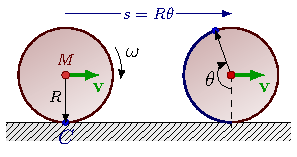
\includegraphics[width=0.5\textwidth]{src/rollingcondition/image1.pdf}
\end{figure}
Per instaurare un \textbf{moto di rotolamento} si può
\begin{enumerate}
  \item applicare una forza all’asse di rotazione
  \item applicare un momento di una forza all’asse
        di rotazione, che come si è visto, è
        equivalente all’applicazione di una coppia
\end{enumerate}
\subsubsection{Condizione di rotolamento puro con \underline{forza applicata}}
Una ruota rotola sotto l’azione di una forza \(\vec{F}\) applicata all’asse di rotazione.\\
La condizione affinché si abbia rotolamento puro senza strisciamento, quindi C sia fermo, è
che la superficie eserciti una forza di attrito statico nel punto C.\\
La \textbf{forza limite applicabile per evitare lo strisciamento} è data da
Scrivendo le equazioni cardinali della dinamica per forze e momenti fissando il polo P in CM si ottiene
\begin{equation*}
  \begin{cases}
    \displaystyle \sum_{i=1}^{N} \vec{F}_i = m \vec{a}_{CM} \\
    \displaystyle \sum_{i=1}^{N} \vec{M}_i = I \vec{\alpha}
  \end{cases}
\end{equation*}

\begin{multicols}{2}
  \textbf{Forze}
  \begin{equation*}
    \vec{F}_{ext} + \vec{F}_{a} + \vec{F}_p + \vec{N} = m \vec{a}_{CM}
  \end{equation*}
  \begin{equation*}
    \begin{cases}
      \text{Lungo x} \\
      \text{Lungo y}
    \end{cases}
  \end{equation*}
  \begin{equation*}
    \begin{cases}
      \vec{F}_{ext} + \vec{F}_{a} = m \vec{a}_{CM} \\
      \vec{F}_p + \vec{N} = 0
    \end{cases}
  \end{equation*}
  \columnbreak
  \noindent
  \\
  \textbf{Momenti} polo in CM (\(P \equiv CM\))
  \begin{equation*}
    \vec{M}_{Fext} + \vec{M}_{Fa} + \vec{M}_{Fp} + \vec{M}_{N} = I \vec{\alpha}
  \end{equation*}
  \begin{equation*}
    F_{ext} \times r_{Fext} - F_{a} \times r_{Fa}  +  - F_p \times r_{Fp} + N \times r_{N} = I \vec{\alpha}
  \end{equation*}
  \begin{equation*}
    F_{ext}  \cdot 0 - F_{a}  r_{Fa} - F_p \cdot 0 + N r_{N} \sin{(180)} = I \vec{\alpha}
  \end{equation*}
  \begin{equation*}
    0 - F_{a} r_{Fa} + 0 + 0 = I \vec{\alpha}
  \end{equation*}
  \begin{equation*}
    - F_{a} r_{Fa} = I \vec{\alpha}
  \end{equation*}
\end{multicols}

\begin{multicols}{2}
  \begin{equation*}
    \begin{cases}
      F_{ext} - F_{a} = m a_{CM} \\
      - F_p + N = 0
    \end{cases}
  \end{equation*}
  \begin{equation*}
    \begin{cases}
      F_{ext} - F_{a} = m a_{CM} \\
      - F_p + N = 0
    \end{cases}
  \end{equation*}
  \begin{equation*}
    \begin{cases}
      F_{ext} - \mu_{as}mg = m a_{CM} \\
      - m g + N = 0
    \end{cases}
  \end{equation*}
  \begin{equation*}
    \begin{cases}
      F_{ext} - F_{a} = m a_{CM} \\
      N = m g
    \end{cases}
  \end{equation*}
  \begin{equation*}
    a_{CM} = \frac{F_{ext} - F_{a}}{m}
  \end{equation*}
  \columnbreak
  \noindent
  \\
  \begin{equation*}
    F_{a} r_{Fa} = - I \vec{\alpha}
  \end{equation*}
  Poiché \(r_{Fa} = r\) e \(\vec{\alpha} = \displaystyle \frac{a_{CM}}{r}\)
  \begin{equation*}
    F_{a} r = - I \frac{a_{CM}}{r}
  \end{equation*}
  \begin{equation*}
    F_{a} = - \frac{I a_{CM}}{r^2}
  \end{equation*}
\end{multicols}
\begin{equation*}
  F_{a} = \displaystyle a_{CM} \frac{I}{r^2}
\end{equation*}
\begin{equation*}
  F_{a} = \displaystyle \frac{F_{ext} - F_{a}}{m} \frac{I}{r^2}
\end{equation*}
\begin{equation*}
  F_{a} = \displaystyle \frac{F_{ext}}{m} \frac{I}{r^2} - \frac{F_{a}}{m} \frac{I}{r^2}
\end{equation*}
\begin{equation*}
  F_{a} = \displaystyle \frac{F_{ext}}{\displaystyle \frac{mr^2}{I} +1}
\end{equation*}
\begin{equation*}
  a_{CM} = \displaystyle \frac{F_{ext}}{m + \displaystyle \frac{I}{r^2}}
\end{equation*}
\begin{equation}
  \boxed{
    \begin{cases}
      \displaystyle a_{CM} = \frac{F_{ext}}{m + \frac{I}{r^2}} \\
      \displaystyle F_{a} = \frac{F_{ext}}{m + \frac{I}{r^2}}
    \end{cases}
  }
\end{equation}
Vi è dunque un limite massimo di forza applicabile affinché si abbia rotolamento puro senza strisciamento che è
\begin{equation*}
  F_{s\ Max} = \mu_s mg
\end{equation*}
\begin{equation*}
  F_{s} \leq F_{s\ Max}
\end{equation*}
\begin{equation*}
  \frac{F_{ext}}{m + \frac{I}{r^2}} \leq \mu_s mg
\end{equation*}
dunque la forza limite applicabile per evitare lo strisciamento è
\begin{equation}
  \boxed{F_{L} = \mu_s mg (\frac{mr^2}{I}+1)}
\end{equation}


\subsubsection{Condizione di rotolamento puro con coppia applicata}
Nella situazione in cui una ruota rotola sotto l’azione di una coppia di forze può essere interpretata come un momento \(\vec{M}_{Fext}\) applicato all’asse di rotazione.\\
\begin{equation*}
  \begin{cases}
    \displaystyle \sum_{i=1}^{N} \vec{F}_i = m \vec{a}_{CM} \\
    \displaystyle \sum_{i=1}^{N} \vec{M}_i = I \vec{\alpha}
  \end{cases}
\end{equation*}
\begin{equation*}
  \begin{cases}
    \vec{F}_{ext\ 1} +\vec{F}_{ext\ 2} + \vec{F}_{a} + \vec{F}_p + \vec{N} = m \vec{a}_{CM} \\
    \vec{M}_{Fext} + \vec{M}_{Fa} + \vec{M}_{Fp} + \vec{M}_{N} = I \vec{\alpha}
  \end{cases}
\end{equation*}
\begin{equation*}
  \begin{cases}
    F_{ext\ 1} -F_{ext\ 2} + F_{a} - F_{p} + N  = m a_{CM} \\
    {M}_{Fext} + M_{Fa} + M_{Fp} + M_{N} = I \alpha
  \end{cases}
\end{equation*}
Poiché il modulo della coppia di forze applicata è uguale \( F_{ext\ 1} = - F_{ext\ 2} \)
\begin{equation*}
  \begin{cases}
    F_{ext\ 1} -F_{ext\ 1} + F_{a} - F_{p} + F_{p}  = m a_{CM} \\
    {M}_{Fext}  + \vec{F}_{a} \times \vec{r}_{Fa} + \vec{F}_{p} \times \vec{r}_{Fp} + \vec{N} \times \vec{r}_{N} = I \vec{\alpha}
  \end{cases}
\end{equation*}
\begin{equation*}
  \begin{cases}
    F_{a} = m a_{CM} \\
    {M}_{Fext} + F_{a} r_{Fa} \sin{270} + F_{p} \cdot 0 + N r_{N} \sin{180} = I \alpha
  \end{cases}
\end{equation*}
\begin{equation*}
  \begin{cases}
    F_{a} = m a_{CM} \\
    {M}_{Fext} - F_{a} r_{Fa} = I \alpha
  \end{cases}
\end{equation*}
Combinandole si ottiene
\begin{equation*}
  \displaystyle {M}_{Fext} - m a_{CM} r_{Fa} = I \alpha
\end{equation*}
\begin{equation*}
  \displaystyle {M}_{Fext} - m a_{CM} r_{Fa} = I \frac{a_{CM}}{r}
\end{equation*}
\begin{equation*}
  \displaystyle a_{CM} = \frac{r_{Fa} M_{Fext}}{I + m r_{Fa}^2}
\end{equation*}
\begin{equation}
  \displaystyle \boxed{a_{CM} = \frac{r M}{I + m r^2}}
\end{equation}
\begin{equation*}
  \displaystyle F_{a} = \frac{m r_{Fa} M_{Fext}}{I + m r_{Fa}^2}
\end{equation*}
\begin{equation}
  \boxed{F_{a} = \frac{m r M}{I + m r^2} = \frac{M}{ r + \frac{I}{m r^2}}}
\end{equation}


La condizione affinché si abbia rotolamento puro senza strisciamento, quindi C sia fermo, è
\begin{equation}
  \boxed{\vec{M} = \mu_s mg (r + \frac{I}{mr})}
\end{equation}

\end{document}

